\documentclass{beamer} 
\usepackage{amsmath,amsthm}
\usepackage{graphicx,microtype,parskip}
\usepackage{caption,subcaption,multirow}
\usepackage{attrib}

\frenchspacing

\usetheme{default}
\usecolortheme{whale}

\setbeamertemplate{navigation symbols}{}

\setbeamercolor{title}{fg=blue,bg=white}

\setbeamercolor{block title}{fg=white,bg=gray}
\setbeamercolor{block body}{fg=black,bg=lightgray}

\setbeamercolor{block title alerted}{fg=white,bg=darkgray}
\setbeamercolor{block body alerted}{fg=black,bg=lightgray}

\AtBeginSection[]
{
  \begin{frame}
    \tableofcontents[currentsection]
  \end{frame}
}


\title{Evolutionary paleoecology and \\the biology of extinction}
\author{Peter D Smits}
\institute{Committee on Evolutionary Biology, University of Chicago}

\begin{document}

%\begin{frame}
%  \begin{quotation}
%    O species, stunned by your terror of chill death, why fear the Styx, why
%    fear the ghosts and empty names, the stuff of poets, the spectres of a
%    phantom world? [\dots] Everything changes, nothing dies: the spirit
%    wanders, arriving here or there, and occupying whatever body it pleases,
%    passing from a wild beast into a human being, from our body into a
%    beast, but is never destroyed. As pliable wax, stamped with new designs,
%    is no longer what it was; does not keep the same form; but is still one
%    and the same.
%    
%    \attrib{Ovid, \underline{Metamorphoses}, book XV: 143-–175}
%  \end{quotation}
%\end{frame}

\begin{frame}
  \maketitle
\end{frame}

\begin{frame}
  \tableofcontents
\end{frame}

\section{Theory}

\begin{frame}
  \frametitle{Framework}

  \begin{alertblock}{Questions}
    \begin{itemize}
      \item Why do certain taxa go extinct while others do not?
      \item How is emergence ``formed?'' When should it be invoked?
      \item Is extinction risk taxon--age independent?
      \item When should we expect global, regional, or local processes to dominate?
    \end{itemize}
  \end{alertblock}
  
\end{frame}

\begin{frame}
  \frametitle{Evolutionary paleoecology}
  \begin{quotation}
    \dots the consequences of distinct ecological factors on differential rate dynamics, particularly rates of faunal turnover and diversification.

    \tiny{\attrib{Kitchell 1985 \textit{Paleobiology}}}
  \end{quotation}

  \vspace{1.3cm}

  \begin{center}
    \begin{tabular}{@{}l@{}}environmental\\interactions\end{tabular} 
    \hspace{1cm}
    \(\rightarrow\) 
    \hspace{1.5cm}
    \begin{tabular}{@{}l@{}}speciation\\extinction\end{tabular}
  \end{center}
\end{frame}

\begin{frame}
  \frametitle{Emergent properties}

  \begin{center}
    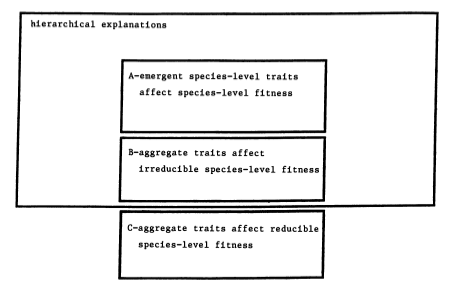
\includegraphics[height=0.4\textheight, width=\textwidth, keepaspectratio=true]{figure/grantham}

    \tiny{\attrib{Grantham 1995 \textit{Ann. Rev. Ecol. Syst.}}}
  \end{center}

  \begin{block}{Criteria}
    Cannot be reduced to lower level (e.g. organismal)
  \end{block}
\end{frame}

\begin{frame}
  \frametitle{Range size}
  
  \begin{center}
    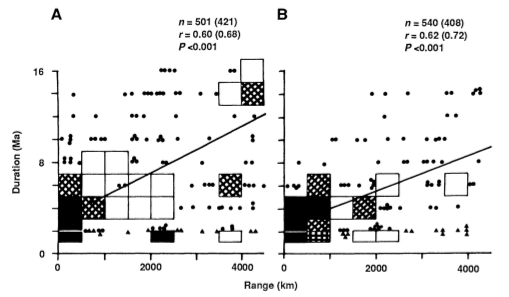
\includegraphics[height = 0.8\textheight, width = \textwidth, keepaspectratio = true]{figure/range}

    \tiny{\attrib{Jablonski 1987 \textit{Science}}}
  \end{center}
\end{frame}

\begin{frame}
  \frametitle{Probability of survival}

  \begin{columns}
    \begin{column}{0.5\textwidth} 
      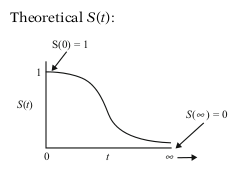
\includegraphics[height = 0.4\textheight, width = \textwidth, keepaspectratio = true]{figure/ideal}

      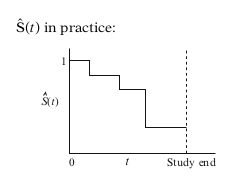
\includegraphics[height = 0.4\textheight, width = \textwidth, keepaspectratio = true]{figure/prac}

      \tiny{\attrib{Kleinbaum and Klein 2012}}
    \end{column}
    \begin{column}{0.5\textwidth}
      \begin{block}{Survival function}
        \[
          S(t) = P(T > t)
        \]

        \begin{itemize}
          \item \(T\): survival time (\(\geq 0\))
          \item \(t\): specified time 
        \end{itemize}
      \end{block}
    \end{column}
  \end{columns}
\end{frame}

\begin{frame}
  \frametitle{Instantaneous potential of failure (extinction)}

  \begin{block}{Hazard function \(\equiv\) conditional failure rate}
    \[
      h(t) = \lim_{\Delta t \to 0} \frac{P(t \leq T < t + \Delta t | T \geq t)}{\Delta t}
    \]
  \end{block}

  \begin{center}
    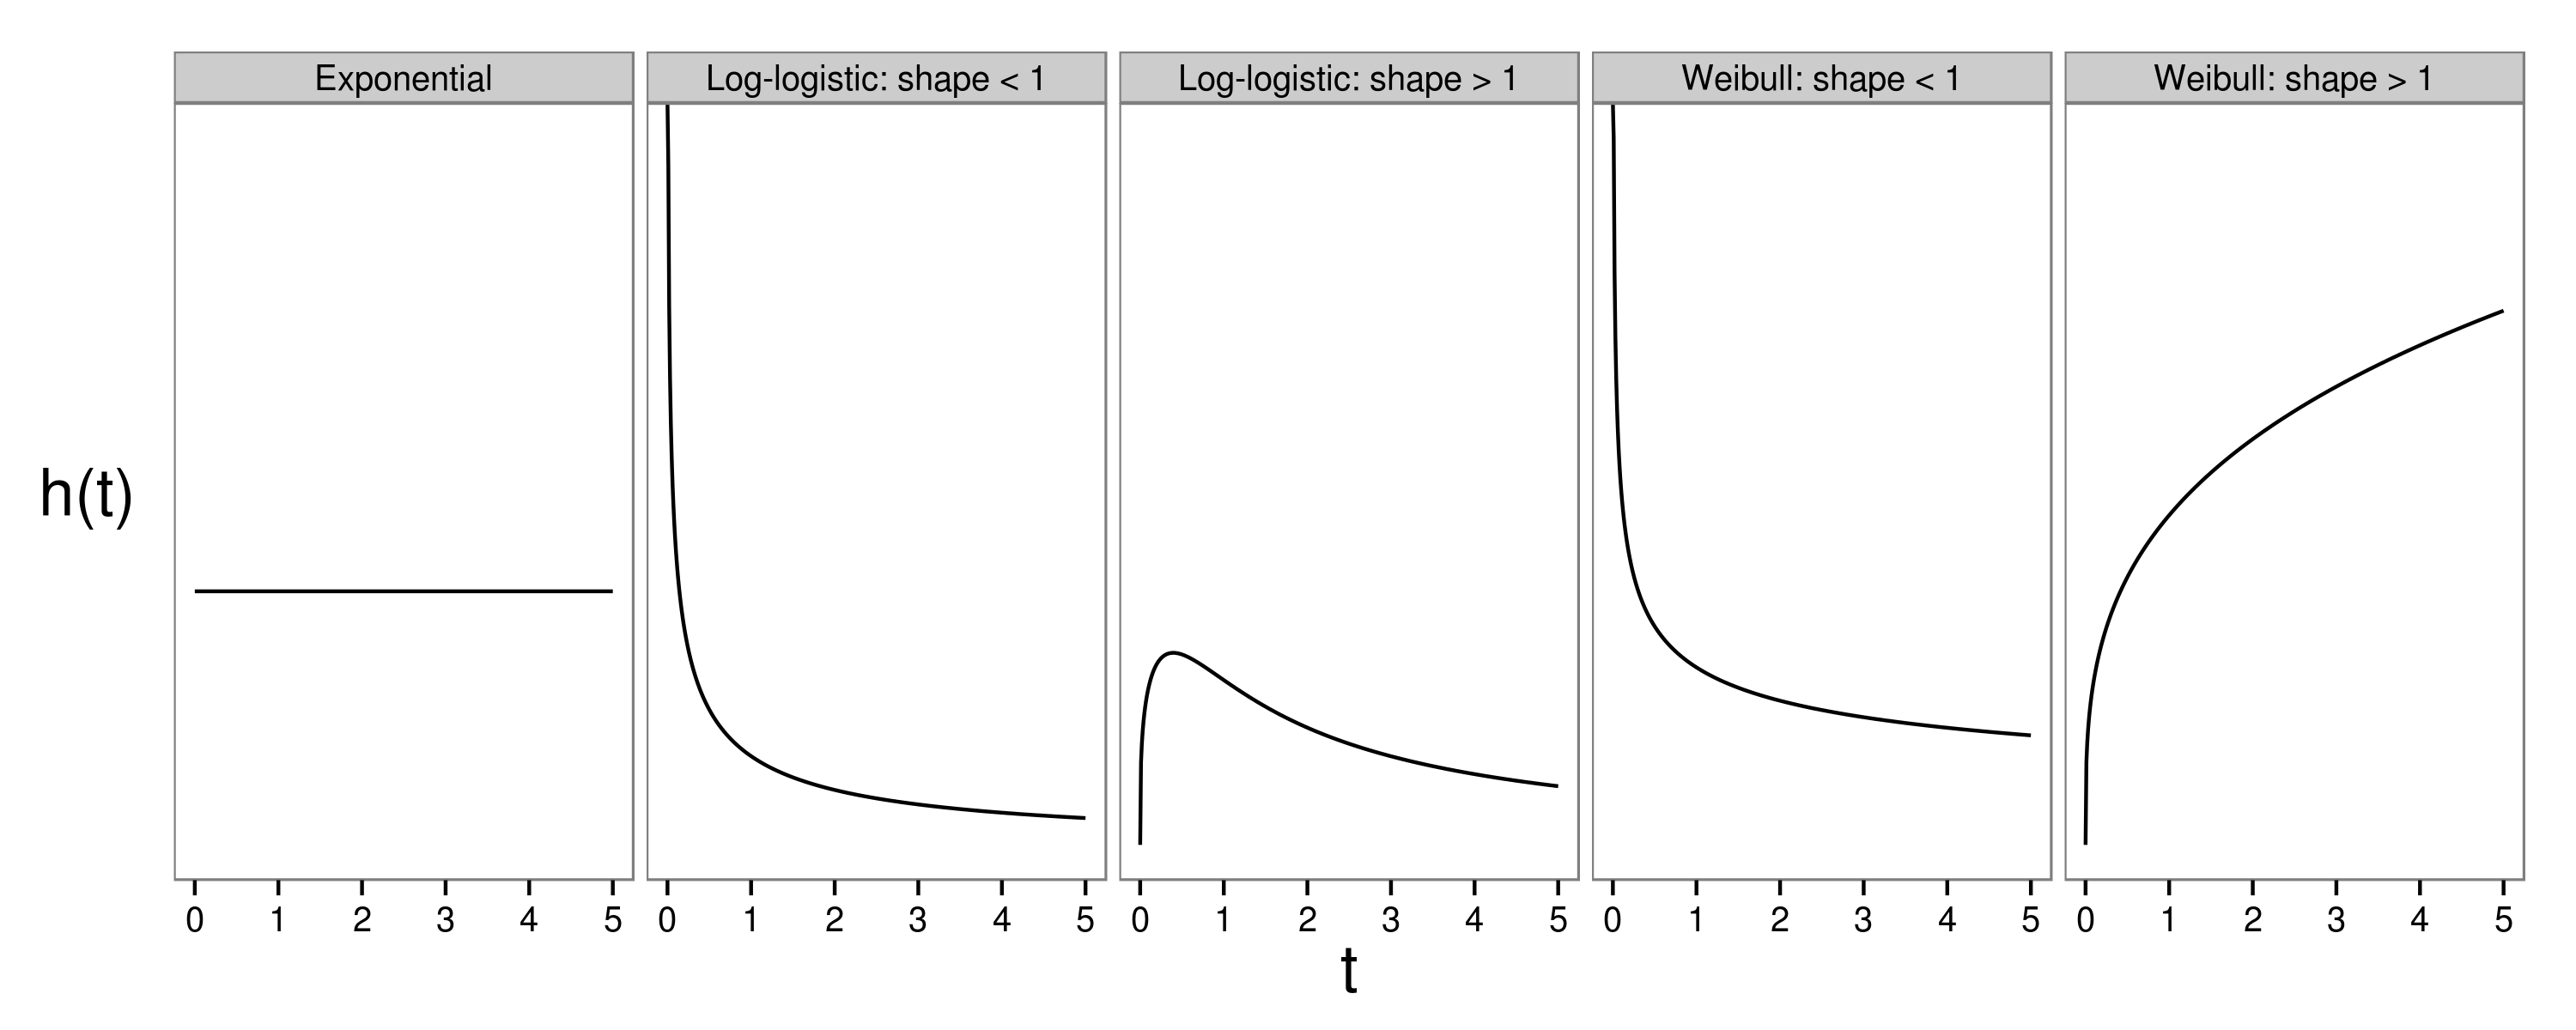
\includegraphics[height = 0.5\textheight, width = \textwidth, keepaspectratio = true]{figure/hazard}
  \end{center}
\end{frame}

\begin{frame}
  \frametitle{Van Valen's observation}

  \begin{center}
    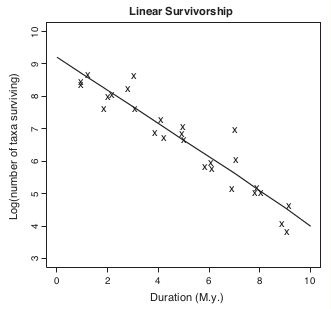
\includegraphics[height = 0.7\textheight, keepaspectratio = true]{figure/liow}

    \tiny{\attrib{Liow et al. 2011 \textit{TREE}}}
  \end{center}
\end{frame}

\begin{frame}
  \frametitle{Law of Constant Extinction}

  \begin{alertblock}{Definition}
      Extinction rate, in a given adaptive zone, is taxon--age independent.

      \tiny{\attrib{Van Valen 1973 \textit{Evol. Theory}}}
  \end{alertblock}

  \begin{center}
    translation: hazard is constant with respect to time \\(\alert{exponential survival})
  \end{center}

  \[
    h(t) = \lambda \iff S(t) = \exp^{-\lambda t}
  \]

\end{frame}

\begin{frame}
  \frametitle{Study systems}

  \begin{columns}
    \begin{column}{0.5\textwidth}
      \begin{block}{brachiopods}
        \begin{itemize}
          \item marine
          \item sessile
          \item Permian (\(\sim 47\) My)
          \item global warming
          \item Australasia
        \end{itemize}
      \end{block}

      \begin{center}
        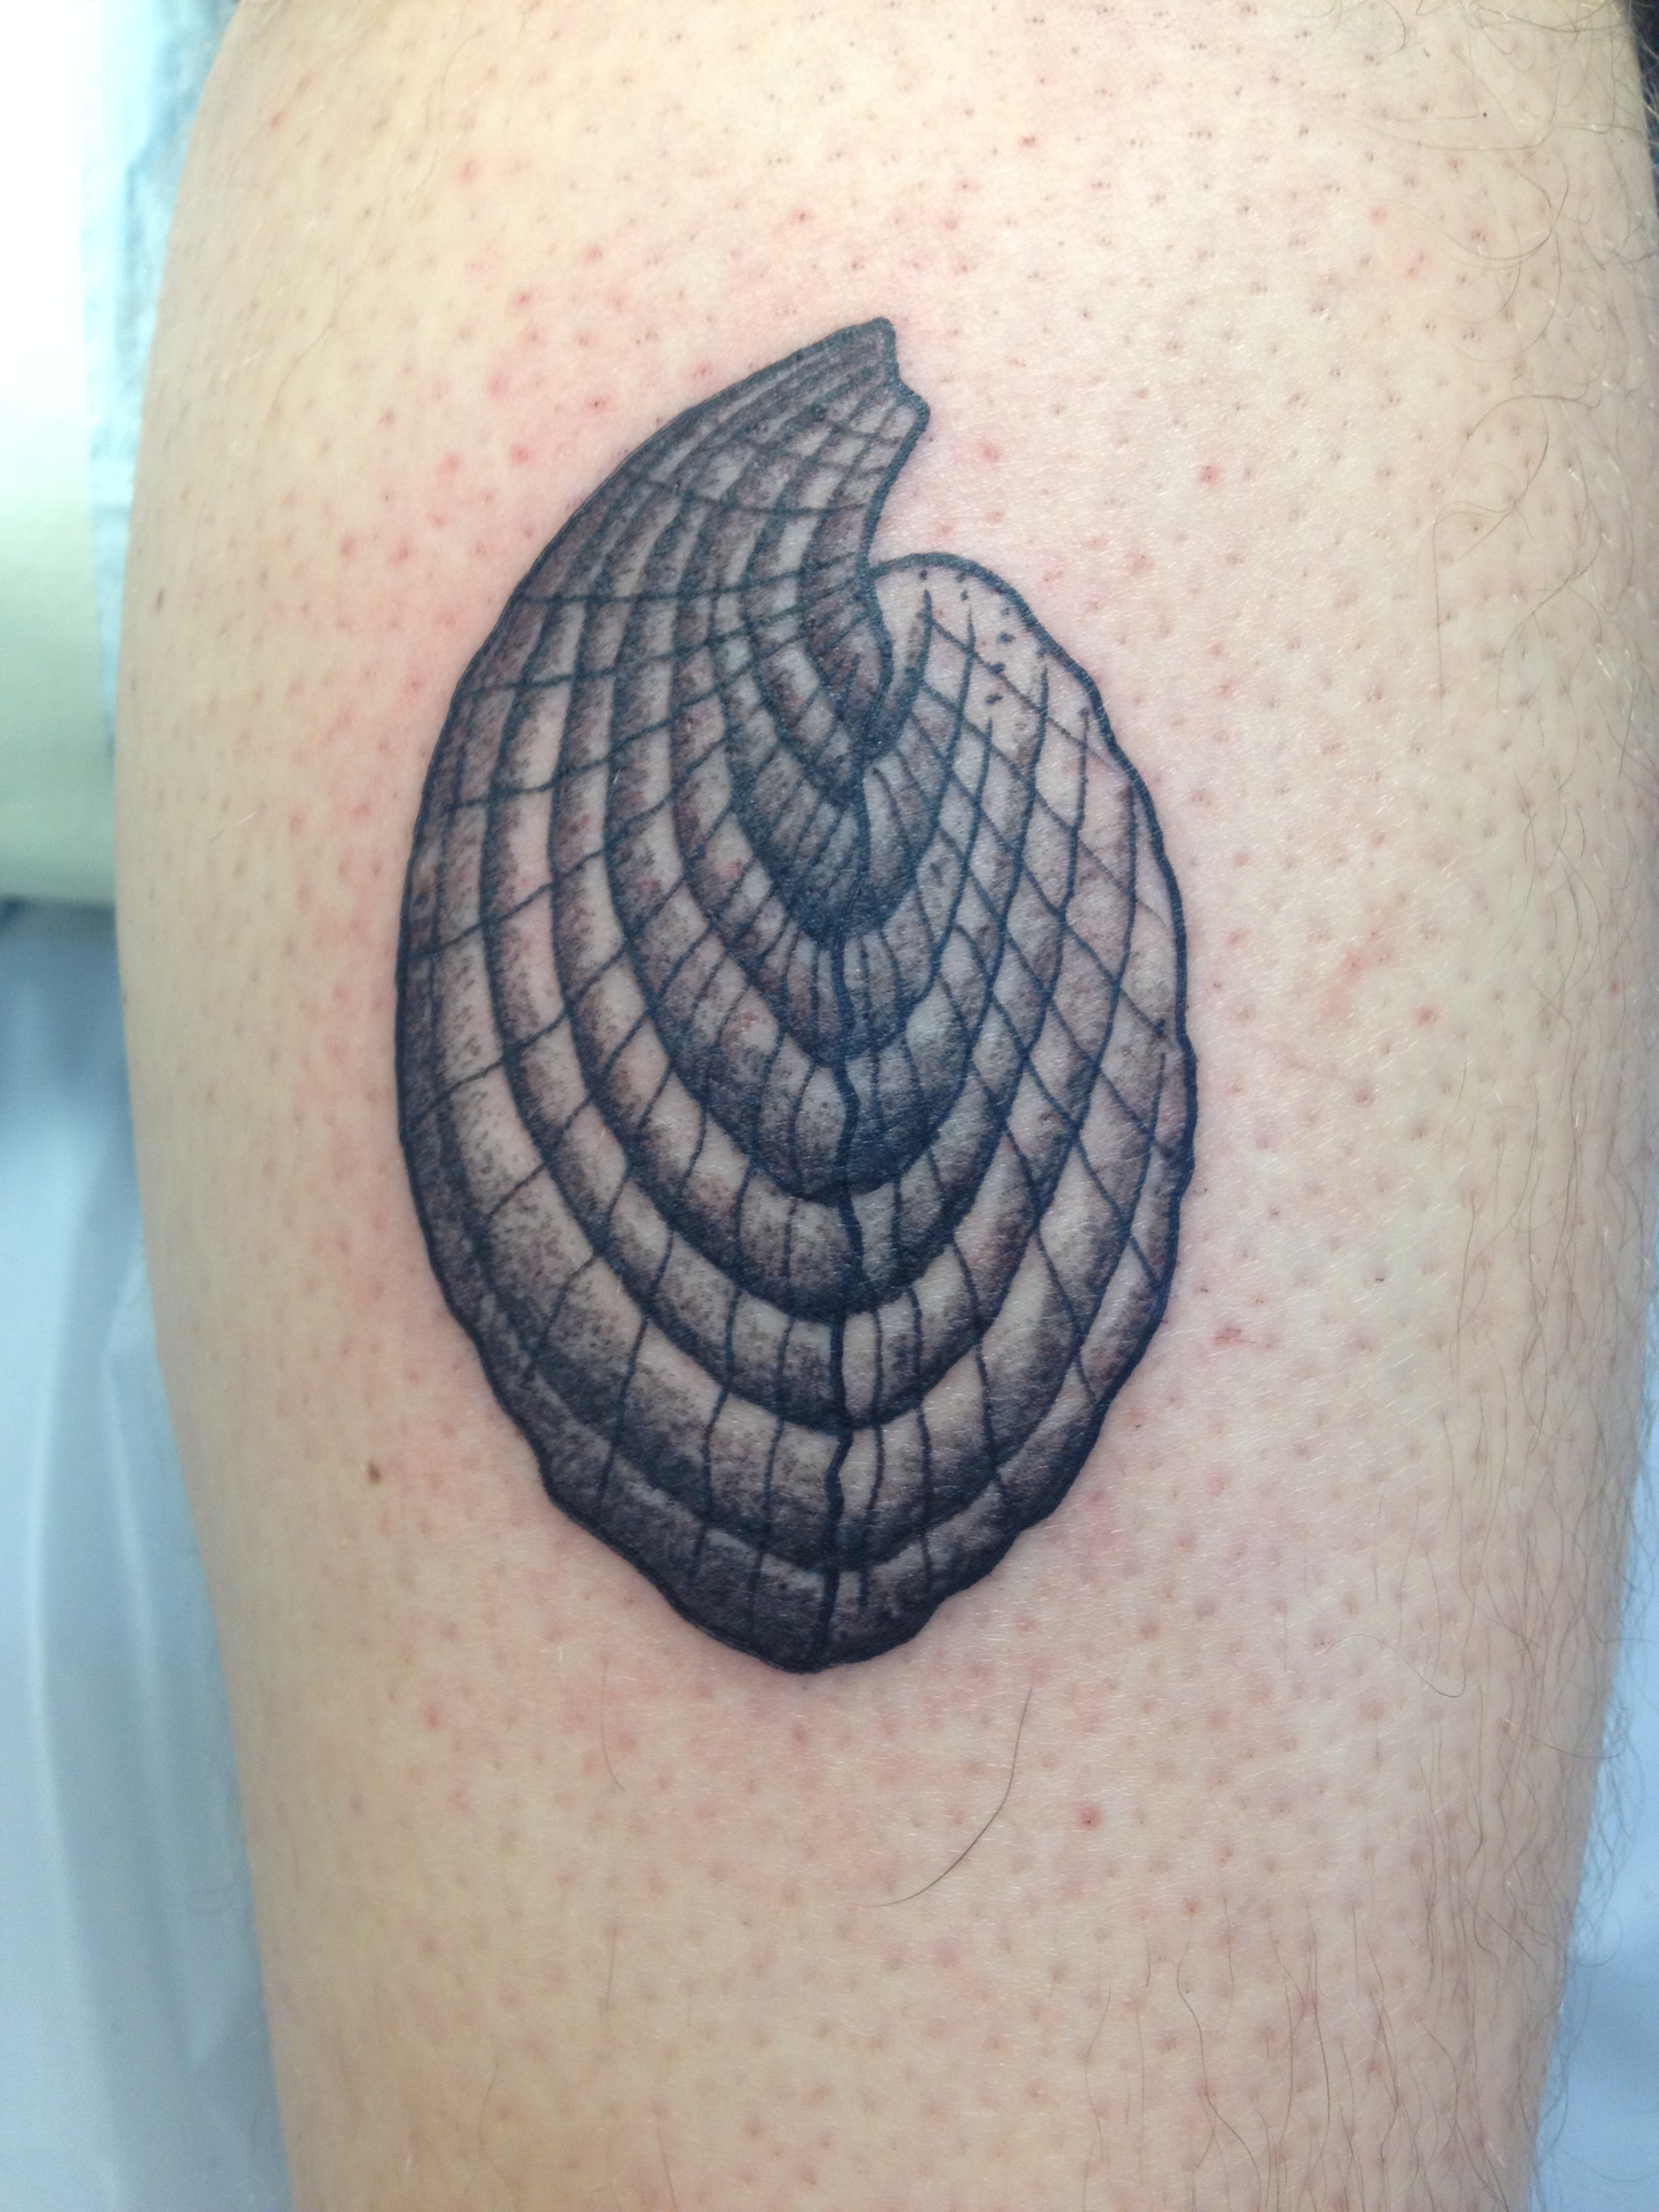
\includegraphics[height = 0.4\textheight, keepaspectratio = true]{figure/tattoo}
      \end{center}
    \end{column}
    \begin{column}{0.5\textwidth}
      \begin{block}{mammals}
        \begin{itemize}
          \item terrestrial
          \item motile
          \item Cenozoic (\(\sim 65\) My)
          \item global cooling
          \item North America, Europe, South America
        \end{itemize}
      \end{block}

      \begin{center}
       
\includegraphics[height = 0.4\textheight, keepaspectratio = true]{figure/annyong}
      \end{center}
    \end{column}
  \end{columns}
\end{frame}

\begin{frame}
  \frametitle{Proposed studies}

  \begin{block}{Chapters}
    \begin{itemize}
      \item Permian brachiopod trait based survival %\\(environmental preference)
        \begin{itemize}
          \item generic level 
          \item necessity of emergence?
        \end{itemize}
      \item Cenozoic mammal trait based survival %\\(range size)
        \begin{itemize}
          \item generic, specific level 
          \item necessity of emergence?
        \end{itemize}
      \item Cenozoic mammal community connectedness %\\(global versus regional versus local)
        \begin{itemize}
          \item global versus regional versus local
          \item differences across traits?
        \end{itemize}
    \end{itemize}
  \end{block}
\end{frame}


\section{Brachiopod survival}

\begin{frame}
  \frametitle{Substrate affinity}

  \begin{columns}
    \begin{column}{0.5\textwidth}
      \begin{center}
        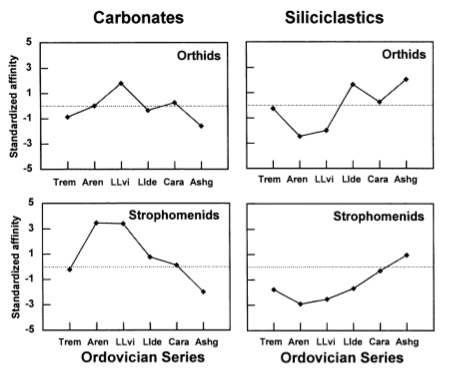
\includegraphics[height = 0.4\textheight, keepaspectratio = true]{figure/miller}
          
        \tiny{\attrib{Miller and Connoly 2001 \textit{Paleobio.}}}

        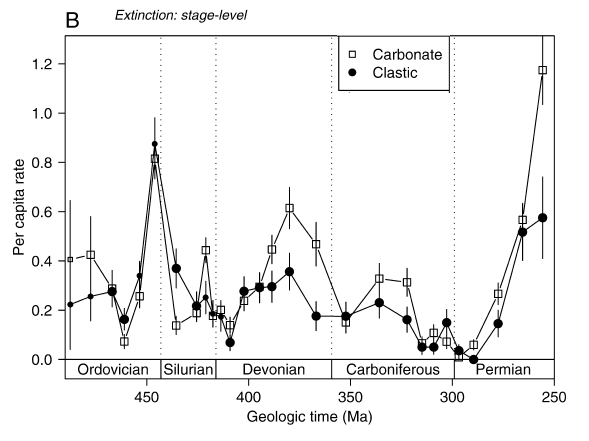
\includegraphics[height = 0.4\textheight, keepaspectratio = true]{figure/foote}
          
        \tiny{\attrib{Foote 2006 \textit{Paleobio.}}}
      \end{center}
    \end{column}
    \begin{column}{0.5\textwidth}
      \begin{itemize}
        \item carbonates, clastics, mixed
          \begin{itemize}
            \item physio-chemical 
            \item availability
            \item weak proxy for \\larval dispersal?
          \end{itemize}
        \item Pharenozoic decrease carbonates:clastics
          \begin{itemize}
            \item predicted longevity: \\clastics \(>\) carbonates
          \end{itemize}
      \end{itemize}
    \end{column}
  \end{columns}
\end{frame}

\begin{frame}
  \frametitle{Habitat preference}

  \begin{columns}
    \begin{column}{0.5\textwidth}
      \begin{center}
        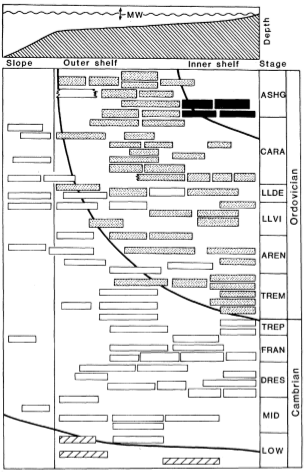
\includegraphics[height = 0.8\textheight, width = \textwidth, keepaspectratio = true]{figure/onoff}

        \tiny{\attrib{Jablonski \textit{et al.} 1983 \textit{Science}}}
      \end{center}
    \end{column}
    \begin{column}{0.5\textwidth}
      \begin{itemize}
        \item on-shore, off-shore, none
          \begin{itemize}
            \item above/below \\storm wave base
            \item energetics, availability
          \end{itemize}
        \item classically invoked re. diversification of higher taxa
          \begin{itemize}
            \item onshore \(\to\) offshore
          \end{itemize}
%        \item Pharenozoic decrease in on-shore:off-shore
%        review in the foote book for better information
      \end{itemize}
    \end{column}
  \end{columns}
\end{frame}

\begin{frame}
  \frametitle{Affixing strategy}

  \begin{columns}
    \begin{column}{0.5\textwidth}
      \begin{center}
        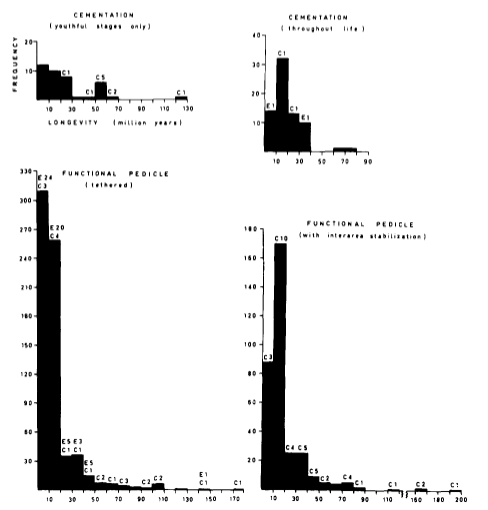
\includegraphics[height = 0.8\textheight, width = \textwidth, keepaspectratio = true]{figure/affix}

        \tiny{\attrib{Alexander 1977 \textit{Paleo\(^3\)}}}
      \end{center}
    \end{column}
    \begin{column}{0.5\textwidth}
      \begin{itemize}
        \item environmental energetics \\and material (mud)
        \item pedunculate, reclining, cementing
          \begin{itemize}
            \item endemics duration: \\reclining \(>\) others
            \item cosmopolitan duration: \\ped./cement \(>\) others
          \end{itemize}
        \item pedunculate:on-shore, reclining:off-shore
      \end{itemize}
    \end{column}
  \end{columns}
\end{frame}

\begin{frame}
  \frametitle{Assigning substrate and habitat}

  \begin{block}{Probability of assignment}
    \begin{align*}
      P(H_{1}|E) &= \frac{P(E|H_{1})P(H_{1})}{P(E|H_{1})P(H_{1}) + P(E|H_{2})P(H_{2})} \\
      P(E|H) &= \binom{n}{k} p^{k}(1 - p)^{n - k}
    \end{align*}

    \begin{itemize}
      \item \(p\): proportion of all collections (e.g) carbonate
      \item \(n\): total \# taxon occurrences
      \item \(k\): of \(n\), \# (e.g.) carbonate occurrences
    \end{itemize}

    \tiny{\attrib{Simpson and Harnik 2009 \textit{Paleobiology}}}
  \end{block}
\end{frame}

\begin{frame}
  \frametitle{Analysis}

  \begin{columns}
    \begin{column}{0.5\textwidth}
      \begin{center}
        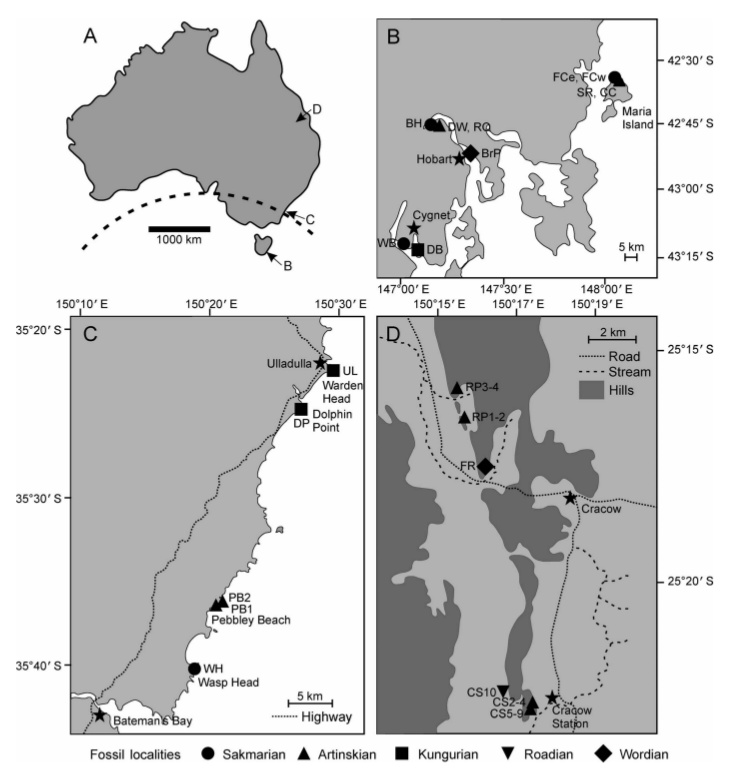
\includegraphics[height = 0.8\textheight, width = \textwidth, keepaspectratio = true]{figure/australia}

        \tiny{\attrib{Clapham and James 2008 \textit{Palaios}}}
      \end{center}
    \end{column}
    \begin{column}{0.5\textwidth}
      \begin{itemize}
        \item genus FAD--LAD
          \begin{itemize}
            \item occurring in, ranging into/out of Permian
            \item interval censoring
          \end{itemize}
        \item time-independent traits
          \begin{itemize}
            \item substrate following Foote 2006 \textit{Paleobio.}
            \item habitat following Kiessling \textit{et al.} 2007 \textit{Paleo\(^3\)}
          \end{itemize}
        \item time-dependent climate 
        \item survival distributions: \(\exp(\lambda)\), \(Weibull(\lambda, k)\), \textit{etc.}
      \end{itemize}
    \end{column}
  \end{columns}
\end{frame}

\begin{frame}
  \frametitle{Preliminary results: model comparison}

  % latex table generated in R 3.0.2 by xtable 1.7-1 package
% Thu Jan  9 14:42:10 2014
\begin{table}[ht]
\centering
\begin{tabular}{llrrrr}
 formula & distribution & shape & df & logLik & AICc \\ 
  \hline
\~{} aff & weibull & 1.91 & 4 & -497.5745 & 1003.4543 \\ 
  \~{} aff + hab & weibull & 1.92 & 6 & -496.8553 & 1006.3618 \\ 
  \~{} aff * hab & weibull & 1.94 & 10 & -495.7702 & 1013.3003 \\ 
  \~{} 1 & weibull & 1.76 & 2 & -515.1666 & 1034.4234 \\ 
  \~{} hab & weibull & 1.76 & 4 & -513.9591 & 1036.2236 \\ 
  \~{} aff & exponential &  & 3 & -532.8690 & 1071.9199 \\ 
  \~{} aff + hab & exponential &  & 5 & -532.5798 & 1075.6211 \\ 
  \~{} 1 & exponential &  & 1 & -540.9218 & 1083.8734 \\ 
  \~{} aff * hab & exponential &  & 9 & -532.3099 & 1084.0485 \\ 
  \~{} hab & exponential &  & 3 & -540.2811 & 1086.7439 \\ 
  \end{tabular}
\label{tab:brach}
\end{table}

\end{frame}

\begin{frame}
  \frametitle{Preliminary results: best substrate}

  \begin{center}
    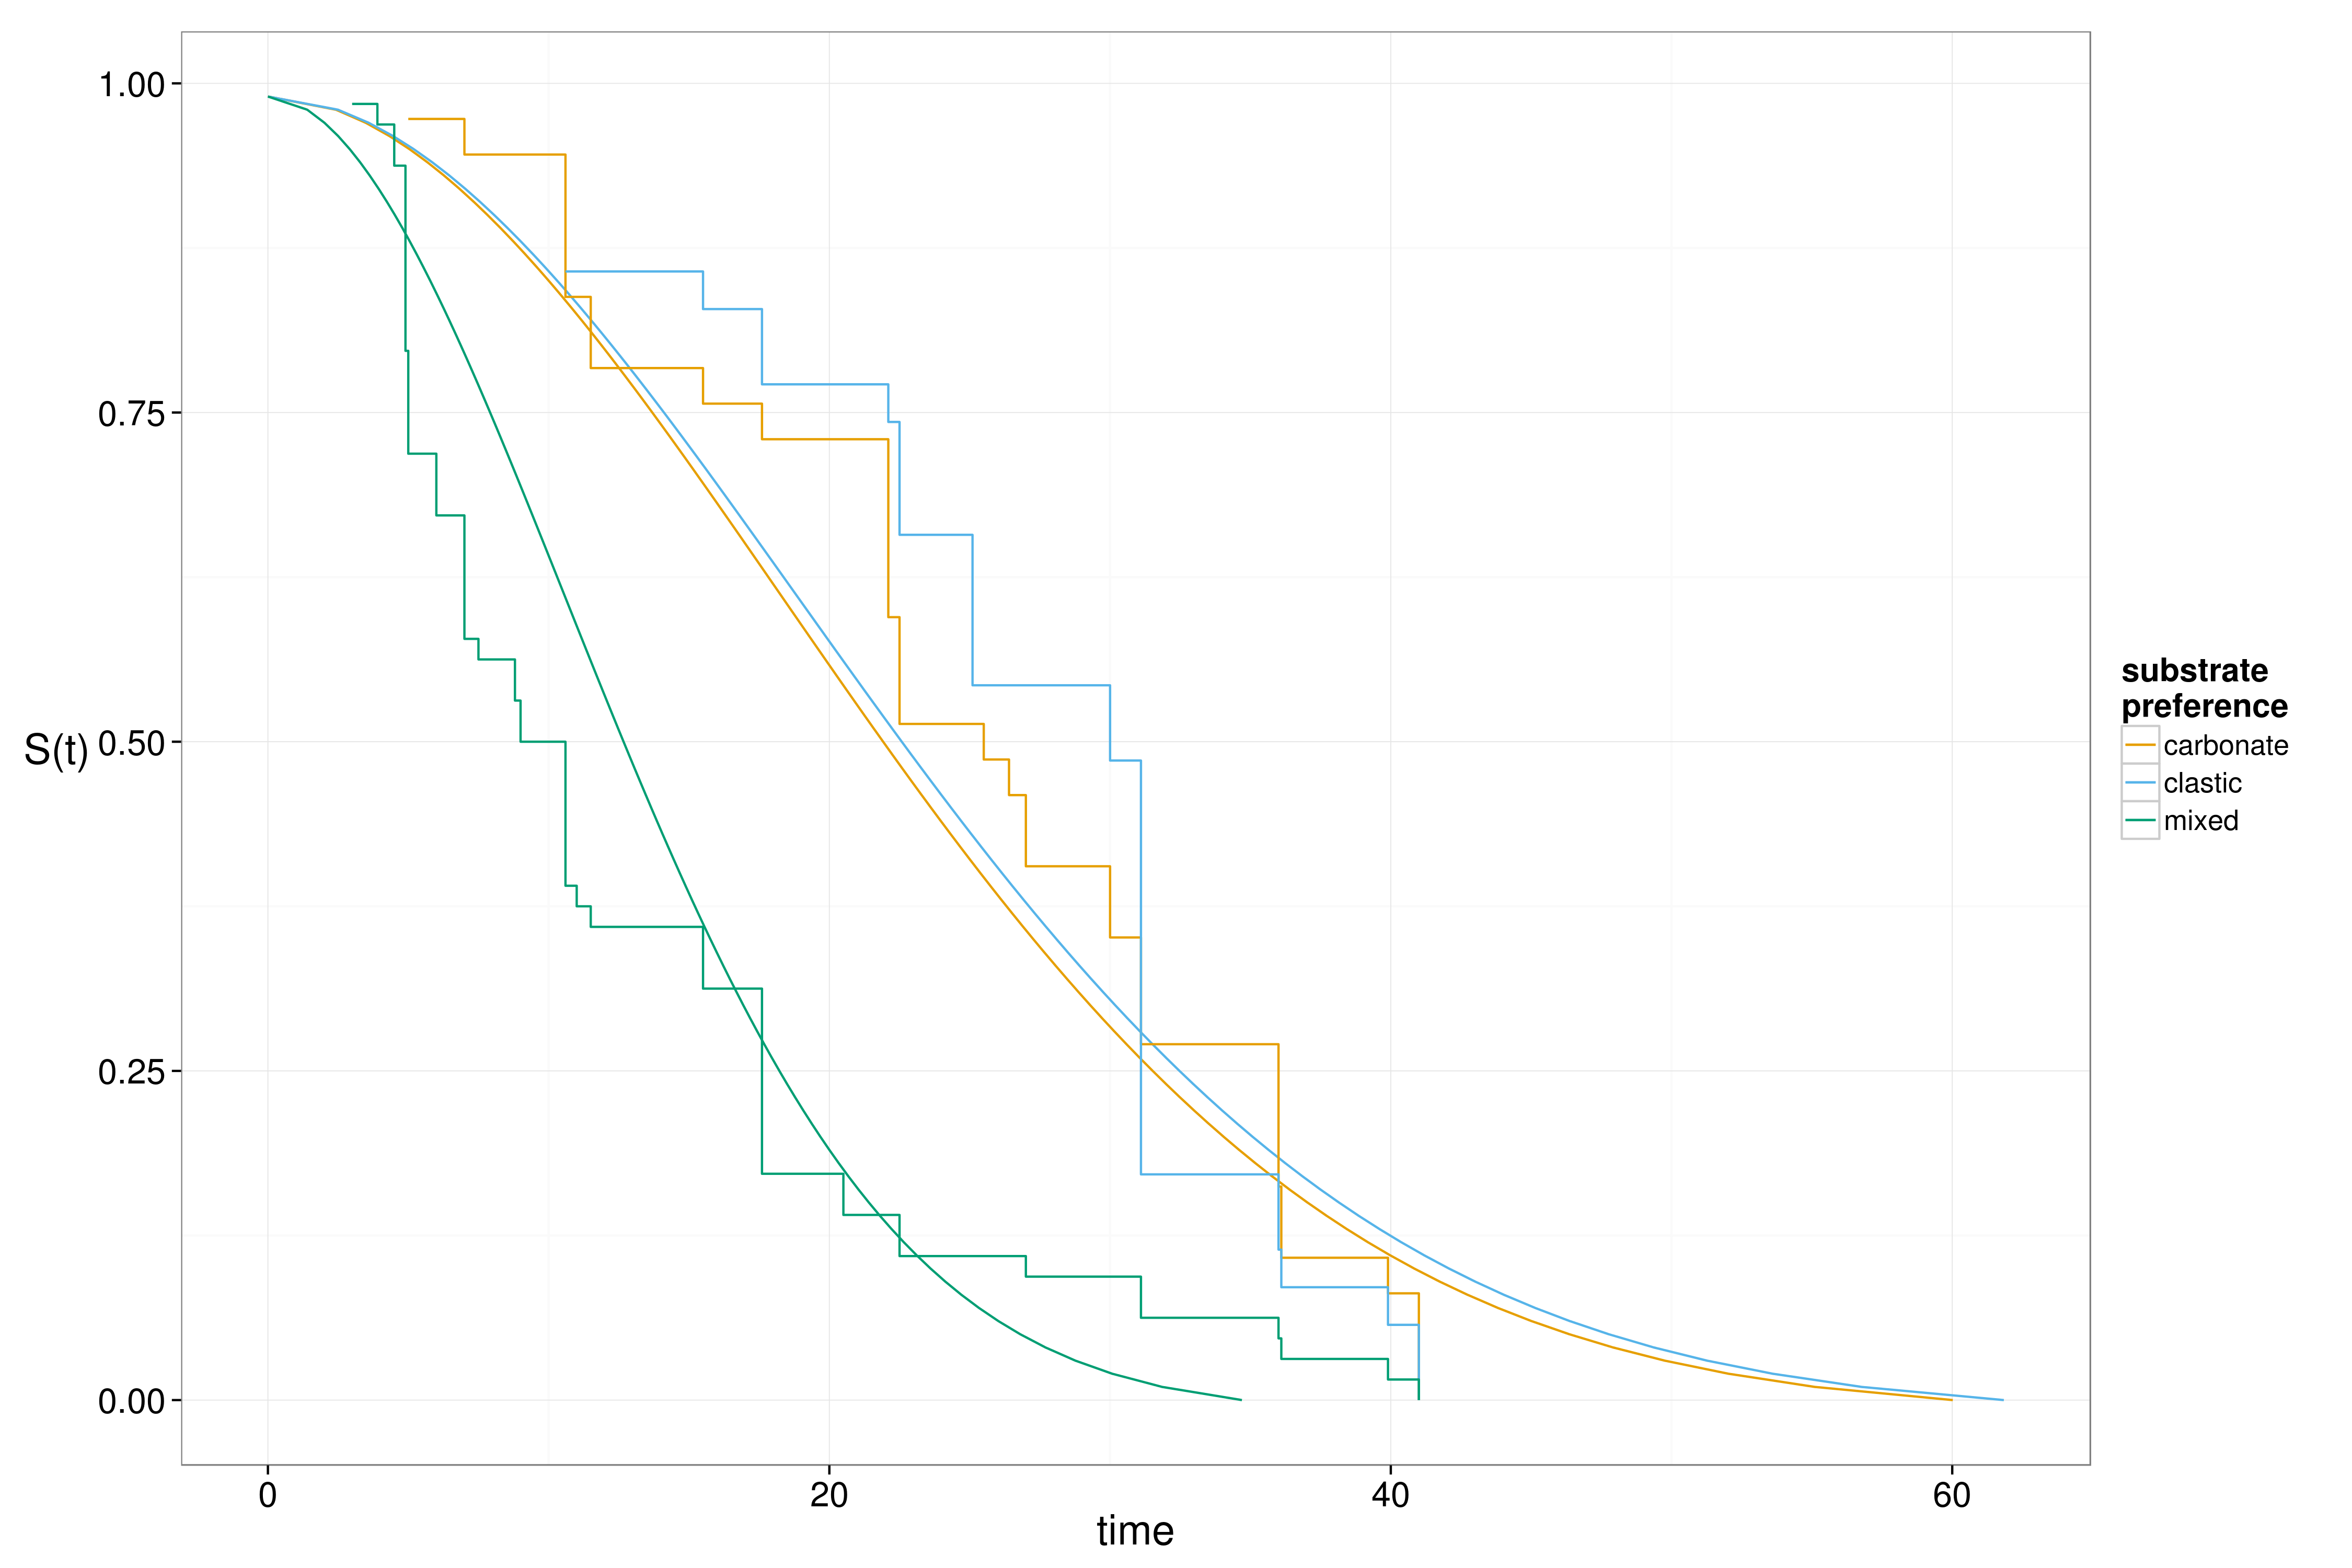
\includegraphics[height = 0.8\textheight, width = \textwidth, keepaspectratio = true]{figure/aff}
  \end{center}
\end{frame}

\begin{frame}
  \frametitle{Preliminary results: best habitat}

  \begin{center}
    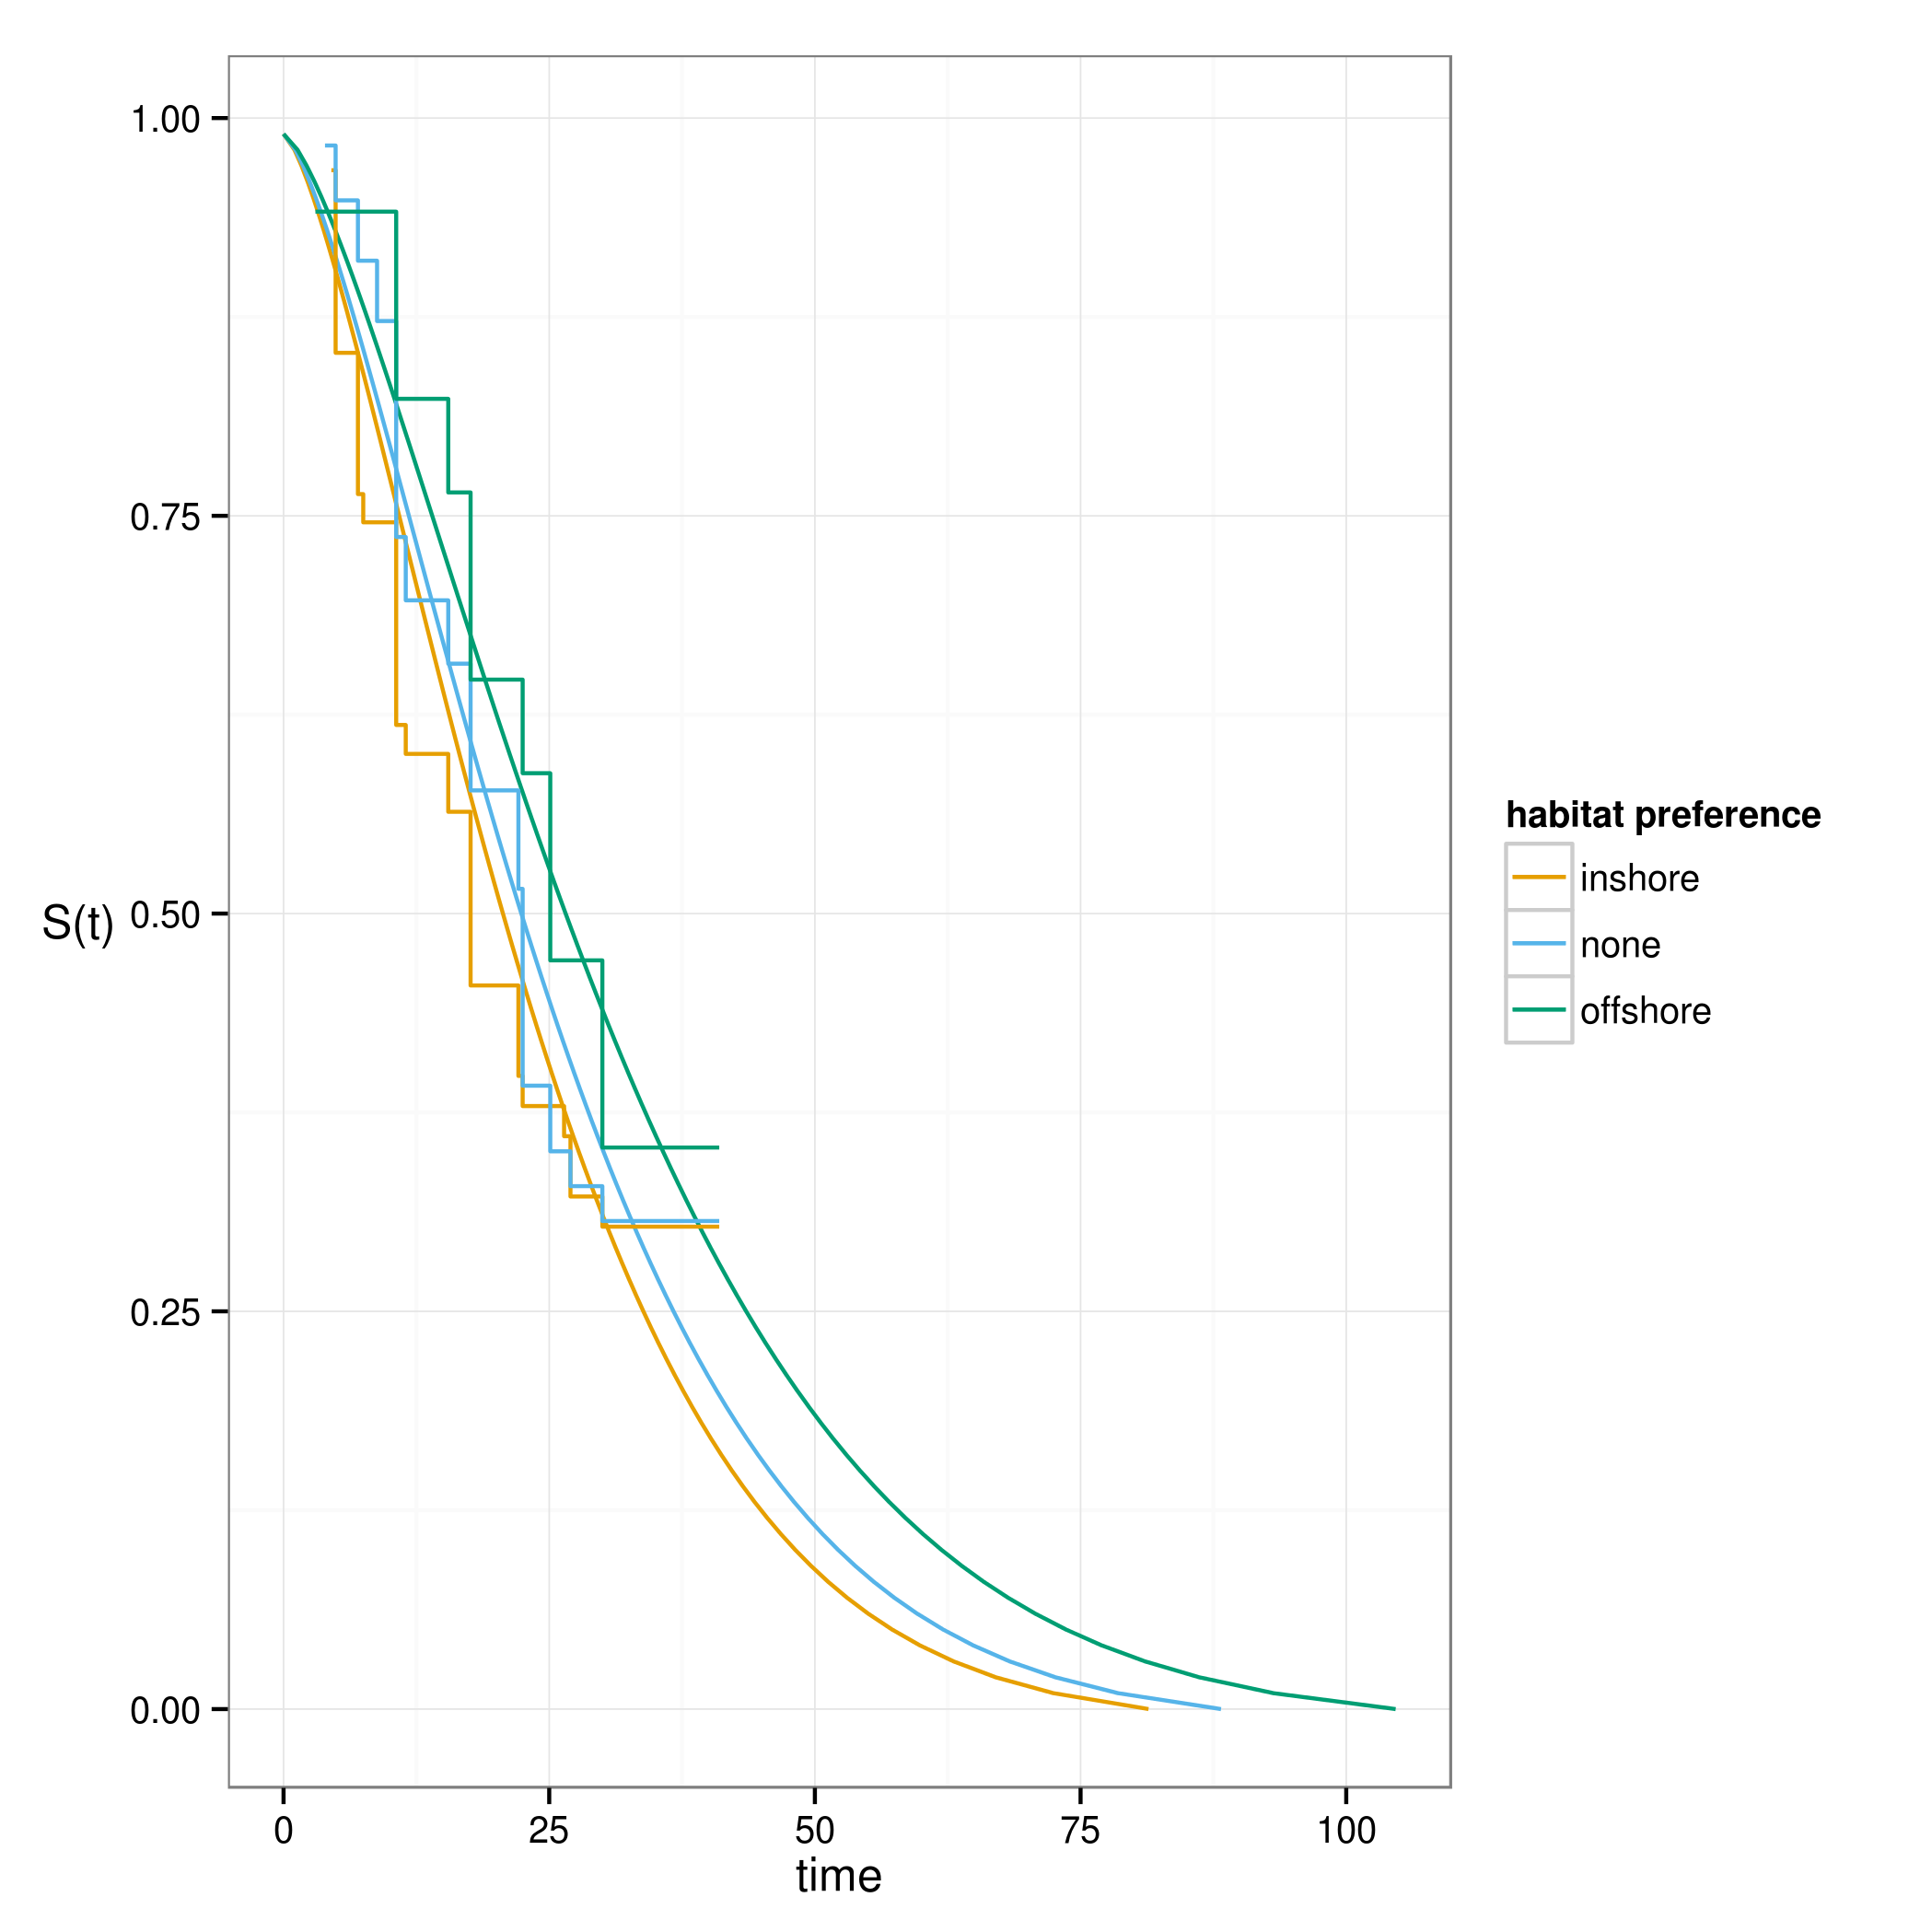
\includegraphics[height = 0.8\textheight, width = \textwidth, keepaspectratio = true]{figure/hab}
  \end{center}
\end{frame}


\section{Mammal survival}

\begin{frame}
  \frametitle{Dietary category}
  \begin{columns}
    \begin{column}{0.5\textwidth}
      \begin{center}
        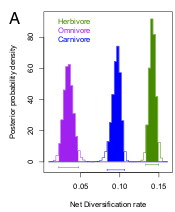
\includegraphics[height=0.4\textheight, width=\textwidth, keepaspectratio=true]{figure/dietdiv}

        \tiny{\attrib{Price \textit{et al.} 2012 \textit{PNAS}}}

        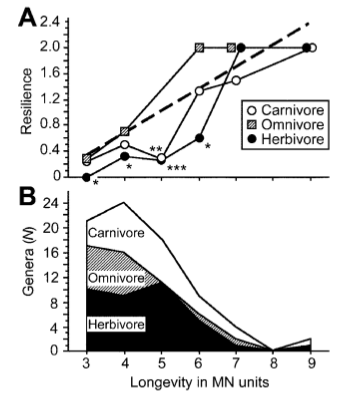
\includegraphics[height=0.4\textheight,width=\textwidth,keepaspectratio=true]{figure/jernvall}

        \tiny{\attrib{Jernvall and Fortelius 2004 \textit{Am. Nat.}}}
      \end{center}
    \end{column}
    \begin{column}{0.5\textwidth}
      \begin{itemize}
        \item trophic hierarchy \\(stability \(\to\) duration)
          \begin{itemize}
            \item herb: most stable, \\longest duration
            \item carni: least stable, \\shortest duration
            \item omni: avg. stability, \\avg. duration
          \end{itemize}
        \item \(\uparrow\) diversification
          \begin{itemize}
            \item \(\uparrow\) origination; \(\simeq\) extinction
            \item \(\simeq\) origination; \(\downarrow\) extinction
          \end{itemize}
      \end{itemize}
    \end{column}
  \end{columns}
\end{frame}

\begin{frame}
  \frametitle{Locomotor category}
  
  \begin{columns}
    \begin{column}{0.5\textwidth}
      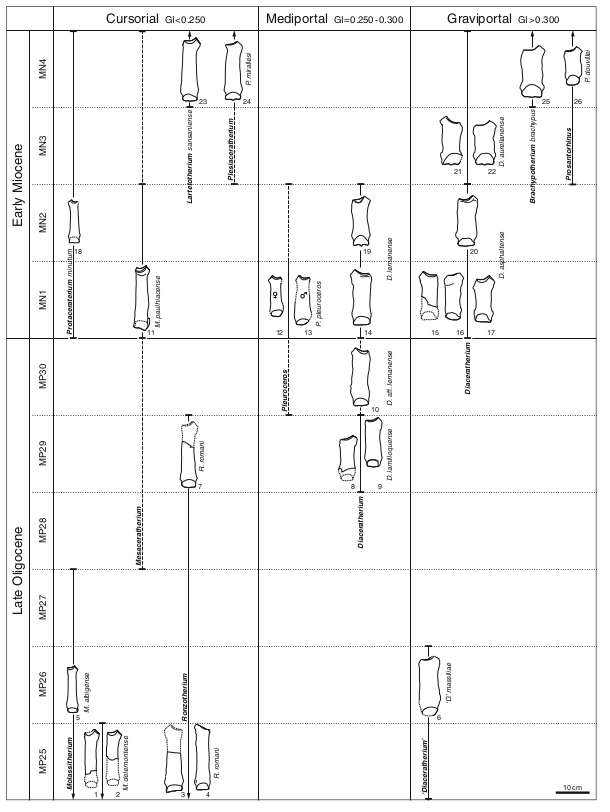
\includegraphics[height=0.8\textheight, width=\textwidth, keepaspectratio=true]{figure/scherler}

      \tiny{\attrib{Scherler \textit{et al.} 2013 \textit{Swiss. J. Geosci.}}}
    \end{column}
    \begin{column}{0.5\textwidth}
      \begin{itemize}
        \item Paleogene \(\to\) Neogene
          \begin{itemize}
            \item open \(\to\) closed environment
          \end{itemize}
        \item predictions
          \begin{itemize}
            \item arboreal: \\Paleogene \(>\) Neogene
            \item ground dwelling: \\Paleogene \(<\) Neogene
            \item scansorial: \\Paleogene \(\approx\) Neogene
          \end{itemize}
      \end{itemize}
    \end{column}
  \end{columns}
\end{frame}

\begin{frame}
  \frametitle{Body size}

  \begin{columns}
    \begin{column}{0.5\textwidth}
      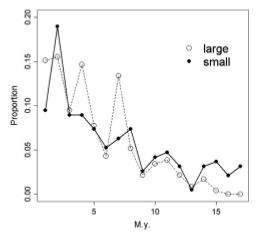
\includegraphics[height=0.4\textheight, width=\textwidth, keepaspectratio=true]{figure/liowmam}

      \tiny{\attrib{Liow \textit{et al.} 2008 \textit{PNAS}}}

      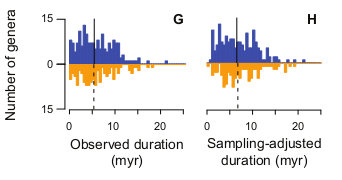
\includegraphics[height=0.4\textheight, width=\textwidth, keepaspectratio=true]{figure/susumu}

      \tiny{\attrib{Tomiya 2013 \textit{Am. Nat.}}}
    \end{column}
    \begin{column}{0.5\textwidth}
      \begin{itemize}
        \item \(\uparrow\) body size, \(\uparrow\) energy req, \\\(\uparrow\) range size, \(\downarrow\) extinction
        \item Europe
          \begin{itemize}
            \item lrg body size genera: \\\(\uparrow\) extinction
          \end{itemize}
        \item North America
          \begin{itemize}
            \item generic body size: \\\(\simeq\) extinction
          \end{itemize}
      \end{itemize}
    \end{column}
  \end{columns}
\end{frame}

\begin{frame}
  \frametitle{Analysis}

  \begin{itemize}
    \item data: genus, species FAD--LAD
      \begin{itemize}
        \item NA: PBDB (h/t Alroy)
        \item Europe: PBDB, NOW
        \item SA: collections, compilations
      \end{itemize}
    \item traits: time-indep. covariates
    \item climate: time-dep. covariate
      \begin{itemize}
        \item continuous \(\delta O^{18}\) isotope (Zachos \textit{et al.} 2008 \textit{Nature})
      \end{itemize}
    \item Paleogene versus Neogene
    \item survival distributions: \(\exp(\lambda)\), \(Weibull(\lambda, k)\), \textit{etc.}
  \end{itemize}
\end{frame}




\section{Mammal community connectedness}

\begin{frame}
  \frametitle{Community connectedness}
  \begin{definition}
    The degree to which localities are composed of endemic versus cosmopolitan taxa, and how similar this ratio is across localities.
  \end{definition}
\end{frame}

\begin{frame}
  \frametitle{Biogeographic networks}
  \begin{columns}
    \begin{column}{0.5\textwidth}
      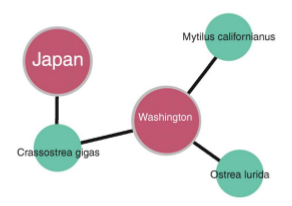
\includegraphics[height = 0.8\textheight, width = \textwidth, keepaspectratio = true]{figure/vilhena}

      \tiny{\attrib{Vilhena \textit{et al.} 2013 \textit{Sci. Reports}}}
    \end{column}
    \begin{column}{0.5\textwidth}
      \begin{itemize}
        \item taxa: species
        \item locality: 2x2 equal--area map projection grid
        \item 2 My intervals
        \item PBDB, NOW, \\museum collections, compilations
      \end{itemize}
    \end{column}
  \end{columns}
\end{frame}

\begin{frame}
  \frametitle{Average relative number of endemics}

  \begin{columns}
    \begin{column}{0.5\textwidth}
      \begin{center}
        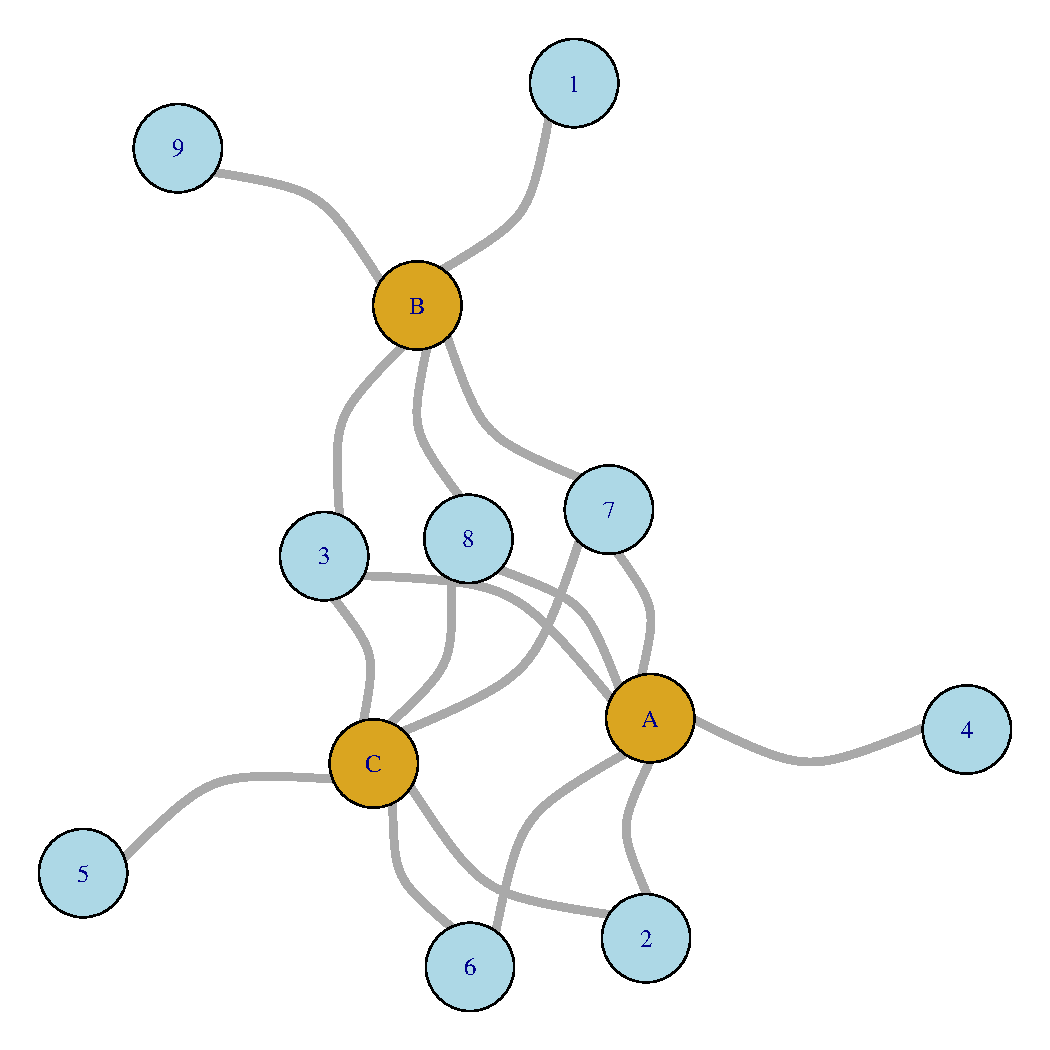
\includegraphics[height = 0.5\textheight, width = \textwidth, keepaspectratio = true]{figure/sim_graph}

        \begin{align*}
          u &= \{1, 2, 1\}\\
          n &= \{6, 5, 6\}\\
          L &= 3\\
          E &\approx 0.24
        \end{align*}
      \end{center}
    \end{column}
    \begin{column}{0.5\textwidth}
      \[
        E = \frac{\sum_{i = 1}^{L} \frac{u_{i}}{n_{i}}}{L}
      \]

      \begin{itemize}
        \item \(L\): number of localities
        \item \(u\): number of taxa unique to a locality
        \item \(n\): number of taxa at a locality
        \item \(0 \leq E \leq 1\)
      \end{itemize}
    \end{column}
  \end{columns}
\end{frame}

\begin{frame}
  \frametitle{Average relative occupancy per taxon}

  \begin{columns}
    \begin{column}{0.5\textwidth}
      \begin{center}
        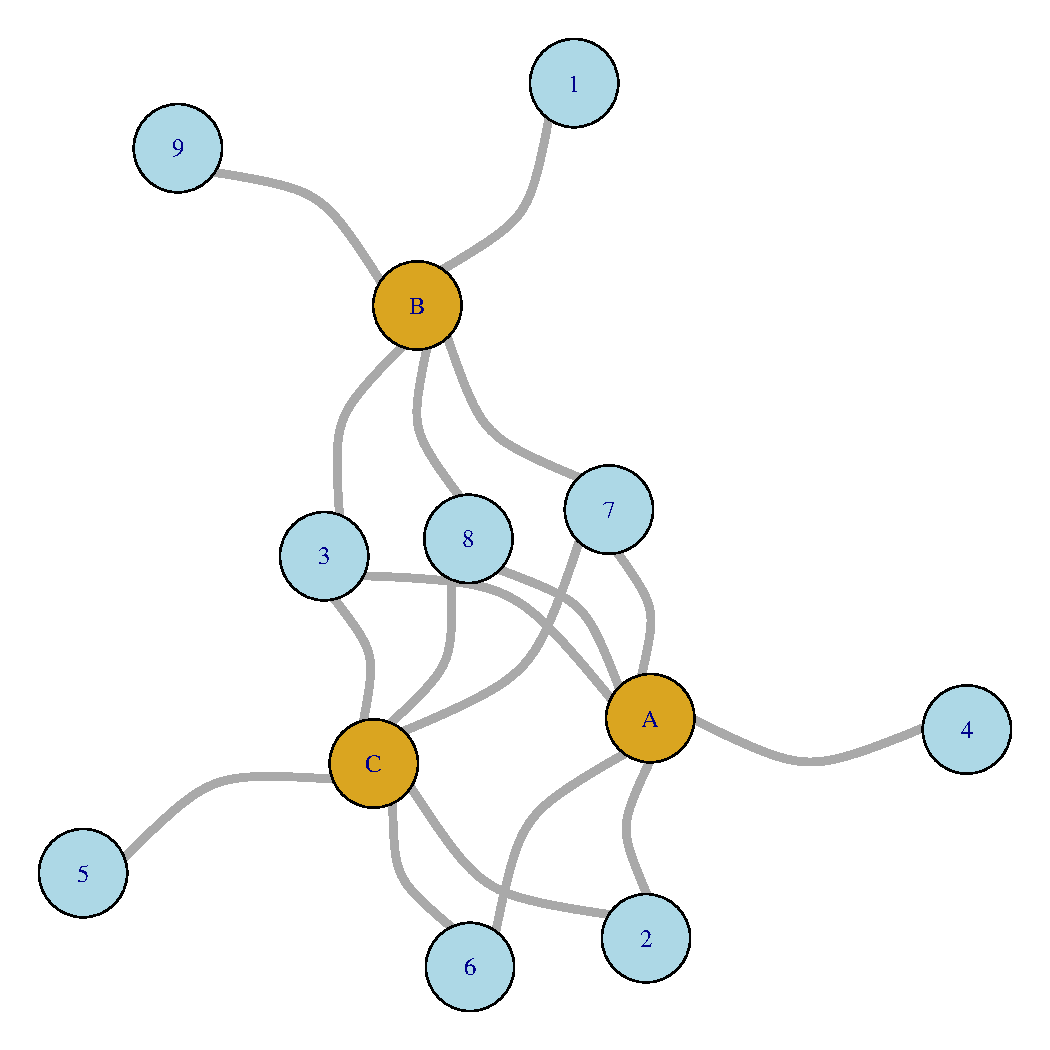
\includegraphics[height = 0.5\textheight, width = \textwidth, keepaspectratio = true]{figure/sim_graph}

        \begin{align*}
          l &= \{1, 2, 3, 1, 1, 2, 3, 3, 1\}\\
          L &= 3\\
          N &= 9\\
          Occ &\approx 0.63 
        \end{align*}
      \end{center}
    \end{column}
    \begin{column}{0.5\textwidth}
      \[
        Occ = \frac{\sum_{i = 1}^{N} \frac{l_{i}}{L}}{N}
      \]

      \begin{itemize}
        \item \(N\): total number of taxa
        \item \(l\): number of localities a taxon occurs at
        \item \(L\): number of localities
        \item \(0 \leq Occ \leq 1\)
      \end{itemize}
    \end{column}
  \end{columns}
\end{frame}

\begin{frame}
  \frametitle{Biogeographic connectedness}

  \begin{columns}
    \begin{column}{0.5\textwidth}
      \begin{center}
        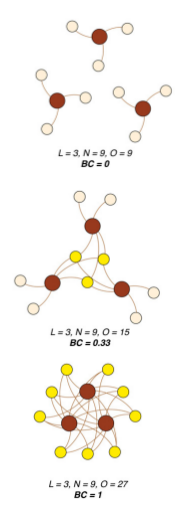
\includegraphics[height=0.8\textheight,width=\textwidth,keepaspectratio=true]{figure/bc}

        \tiny{\attrib{Sidor et al. 2013 \textit{PNAS}}}
      \end{center}
    \end{column}
    \begin{column}{0.5\textwidth}
      \[
        BC = \frac{O - N}{LN - N}
      \]

      \begin{itemize}
        \item \(O\): number of occurrences
        \item \(N\): total number of taxa
        \item \(L\): number of localities
        \item \(0 \leq BC \leq 1\)
      \end{itemize}
    \end{column}
  \end{columns}
\end{frame}

\begin{frame}
  \frametitle{Code length}
  \begin{center}
    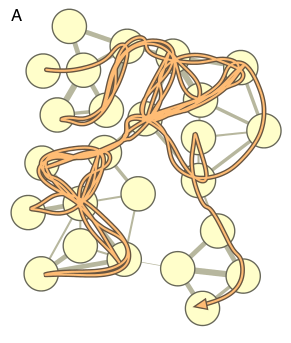
\includegraphics[height=0.8\textheight,width=\textwidth,keepaspectratio=true]{figure/map1}

    \tiny{\attrib{Rosvall and Bergstrom 2008 \textit{PNAS}}}
  \end{center}
\end{frame}

\begin{frame}
  \frametitle{Code length}
  \begin{center}
    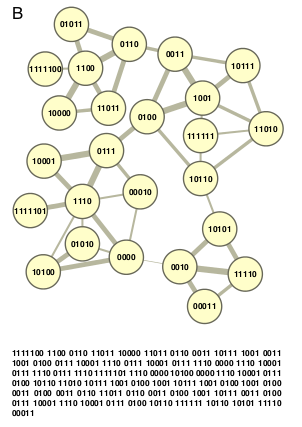
\includegraphics[height=0.8\textheight,width=\textwidth,keepaspectratio=true]{figure/map2}

    \tiny{\attrib{Rosvall and Bergstrom 2008 \textit{PNAS}}}
  \end{center}
\end{frame}

\begin{frame}
  \frametitle{Code length}
  \begin{center}
    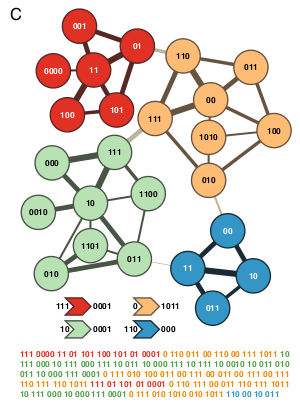
\includegraphics[height=0.8\textheight,width=\textwidth,keepaspectratio=true]{figure/map3}

    \tiny{\attrib{Rosvall and Bergstrom 2008 \textit{PNAS}}}
  \end{center}
\end{frame}

\begin{frame}
  \frametitle{Code length}
  \begin{center}
    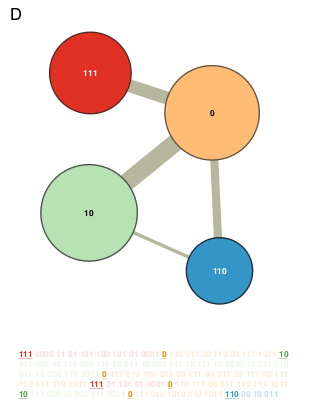
\includegraphics[height=0.8\textheight,width=\textwidth,keepaspectratio=true]{figure/map4}

    \tiny{\attrib{Rosvall and Bergstrom 2008 \textit{PNAS}}}

  \end{center}
\end{frame}

\begin{frame}
  \frametitle{Compressing a network}

  \begin{block}{Map equation \attrib{Rosvall and Bargstrom 2008 \textit{PNAS}}}
    \begin{align*}
      L(\textbf{M}) &= q_{\curvearrowright}H(\mathcal{Q}) + \sum^{m}_{i = 1} p^{i}_{\circlearrowright}H(\mathcal{P}^{i})
    \end{align*}

    \begin{itemize}
      \item \(\textbf{M}\): module partion of \textit{n} nodes in \textit{m} partitions
      \item \(L(\textbf{M})\): code length of network
      \item \(q_{\curvearrowright}\): P(random walk switches modules)
      \item \(H(\mathcal{Q})\): entropy module codewords
      \item \(H(\mathcal{P}^{i})\): entropy within--module
      \item \(p^{i}_{\circlearrowright}\): rate of within--module use
    \end{itemize}
  \end{block}
\end{frame}


\begin{frame}
  \frametitle{Global versus regional versus local scale}

  \begin{columns}
    \begin{column}{0.55\textwidth}
      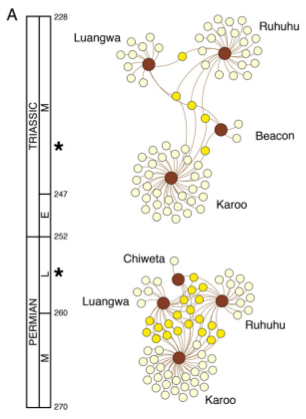
\includegraphics[height=0.7\textheight,width=\textwidth,keepaspectratio=true]{figure/permian}

      \tiny{\attrib{Sidor et al. 2013 \textit{PNAS}}}
    \end{column}
    \begin{column}{0.45\textwidth}
      \begin{itemize}
        \item global
          \begin{itemize}
            \item corr w/ global climate
            \item multiple regions corr
          \end{itemize}
        \item regional
          \begin{itemize}
            \item \(\downarrow E\), \(\uparrow Occ\), \\\(\uparrow BC\), \(\uparrow\) code
          \end{itemize}
        \item local
          \begin{itemize}
            \item \(\uparrow E\), \(\downarrow Occ\), \\\(\downarrow BC\), \(\downarrow\) code
          \end{itemize}
        \item \alert{not mutually exclusive}
      \end{itemize}
    \end{column}
  \end{columns}
\end{frame}

\begin{frame}
  \frametitle{Global expectations: locomotor category}

  \begin{columns}
    \begin{column}{0.6\textwidth}
      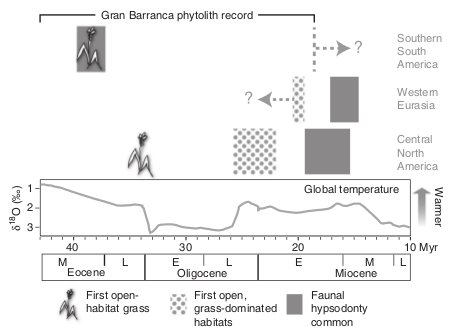
\includegraphics[height=0.8\textheight,width=\textwidth,keepaspectratio=true]{figure/stromberg}

      \tiny{\attrib{Str\"{o}mberg \textit{et al.} 2013 \textit{Nature Com.}}}
    \end{column}
    \begin{column}{0.4\textwidth}
      \begin{itemize}
        \item arboreal
          \begin{itemize}
            \item \(\uparrow E\), \(\uparrow\) code
            \item \(\downarrow BC\), \(\downarrow Occ\)
          \end{itemize}
        \item ground dwelling
          \begin{itemize}
            \item \(\downarrow E\), \(\downarrow\) code
            \item \(\uparrow BC\), \(\uparrow Occ\)
          \end{itemize}
        \item scansorial
          \begin{itemize}
            \item constant \(\lor\) random
          \end{itemize}
      \end{itemize}
    \end{column}
  \end{columns}
\end{frame}

\begin{frame}
  \frametitle{Global expectations: dietary category}

  \begin{columns}
    \begin{column}{0.6\textwidth}
      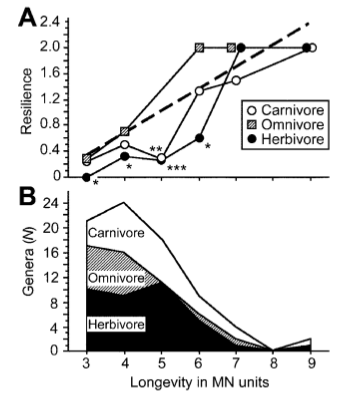
\includegraphics[height=0.7\textheight,width=\textwidth,keepaspectratio=true]{figure/jernvall}

      \tiny{\attrib{Jernvall and Fortelius 2004 \textit{Am. Nat.}}}
    \end{column}
    \begin{column}{0.4\textwidth}
      \begin{itemize}
        \item herbivore
          \begin{itemize}
            \item most like all taxa
          \end{itemize}
        \item carnivore
          \begin{itemize}
            \item constant \(\lor\) corr w/ herbivores
          \end{itemize}
        \item omnivore
          \begin{itemize}
            \item constant \(\lor\) random
          \end{itemize}
      \end{itemize}
    \end{column}
  \end{columns}
\end{frame}

\begin{frame}
  \frametitle{Regional variation} 
  % this is the weakest slide in the entire presentation

  \begin{itemize}
    \item North America
      \begin{itemize}
        \item similar to global predictions
        \item major lit. questions re. effects climate change
      \end{itemize}
    \item Europe
      \begin{itemize}
        \item stable trophic diversity
        \item abundant herbivores drive patterns
      \end{itemize}
    \item South America
      \begin{itemize}
        \item high provincialism
        \item early expansion of ground dwelling taxa
      \end{itemize}
  \end{itemize}
\end{frame}

\begin{frame}
  \frametitle{Preliminary results: NA, Eur}

  \begin{center}
    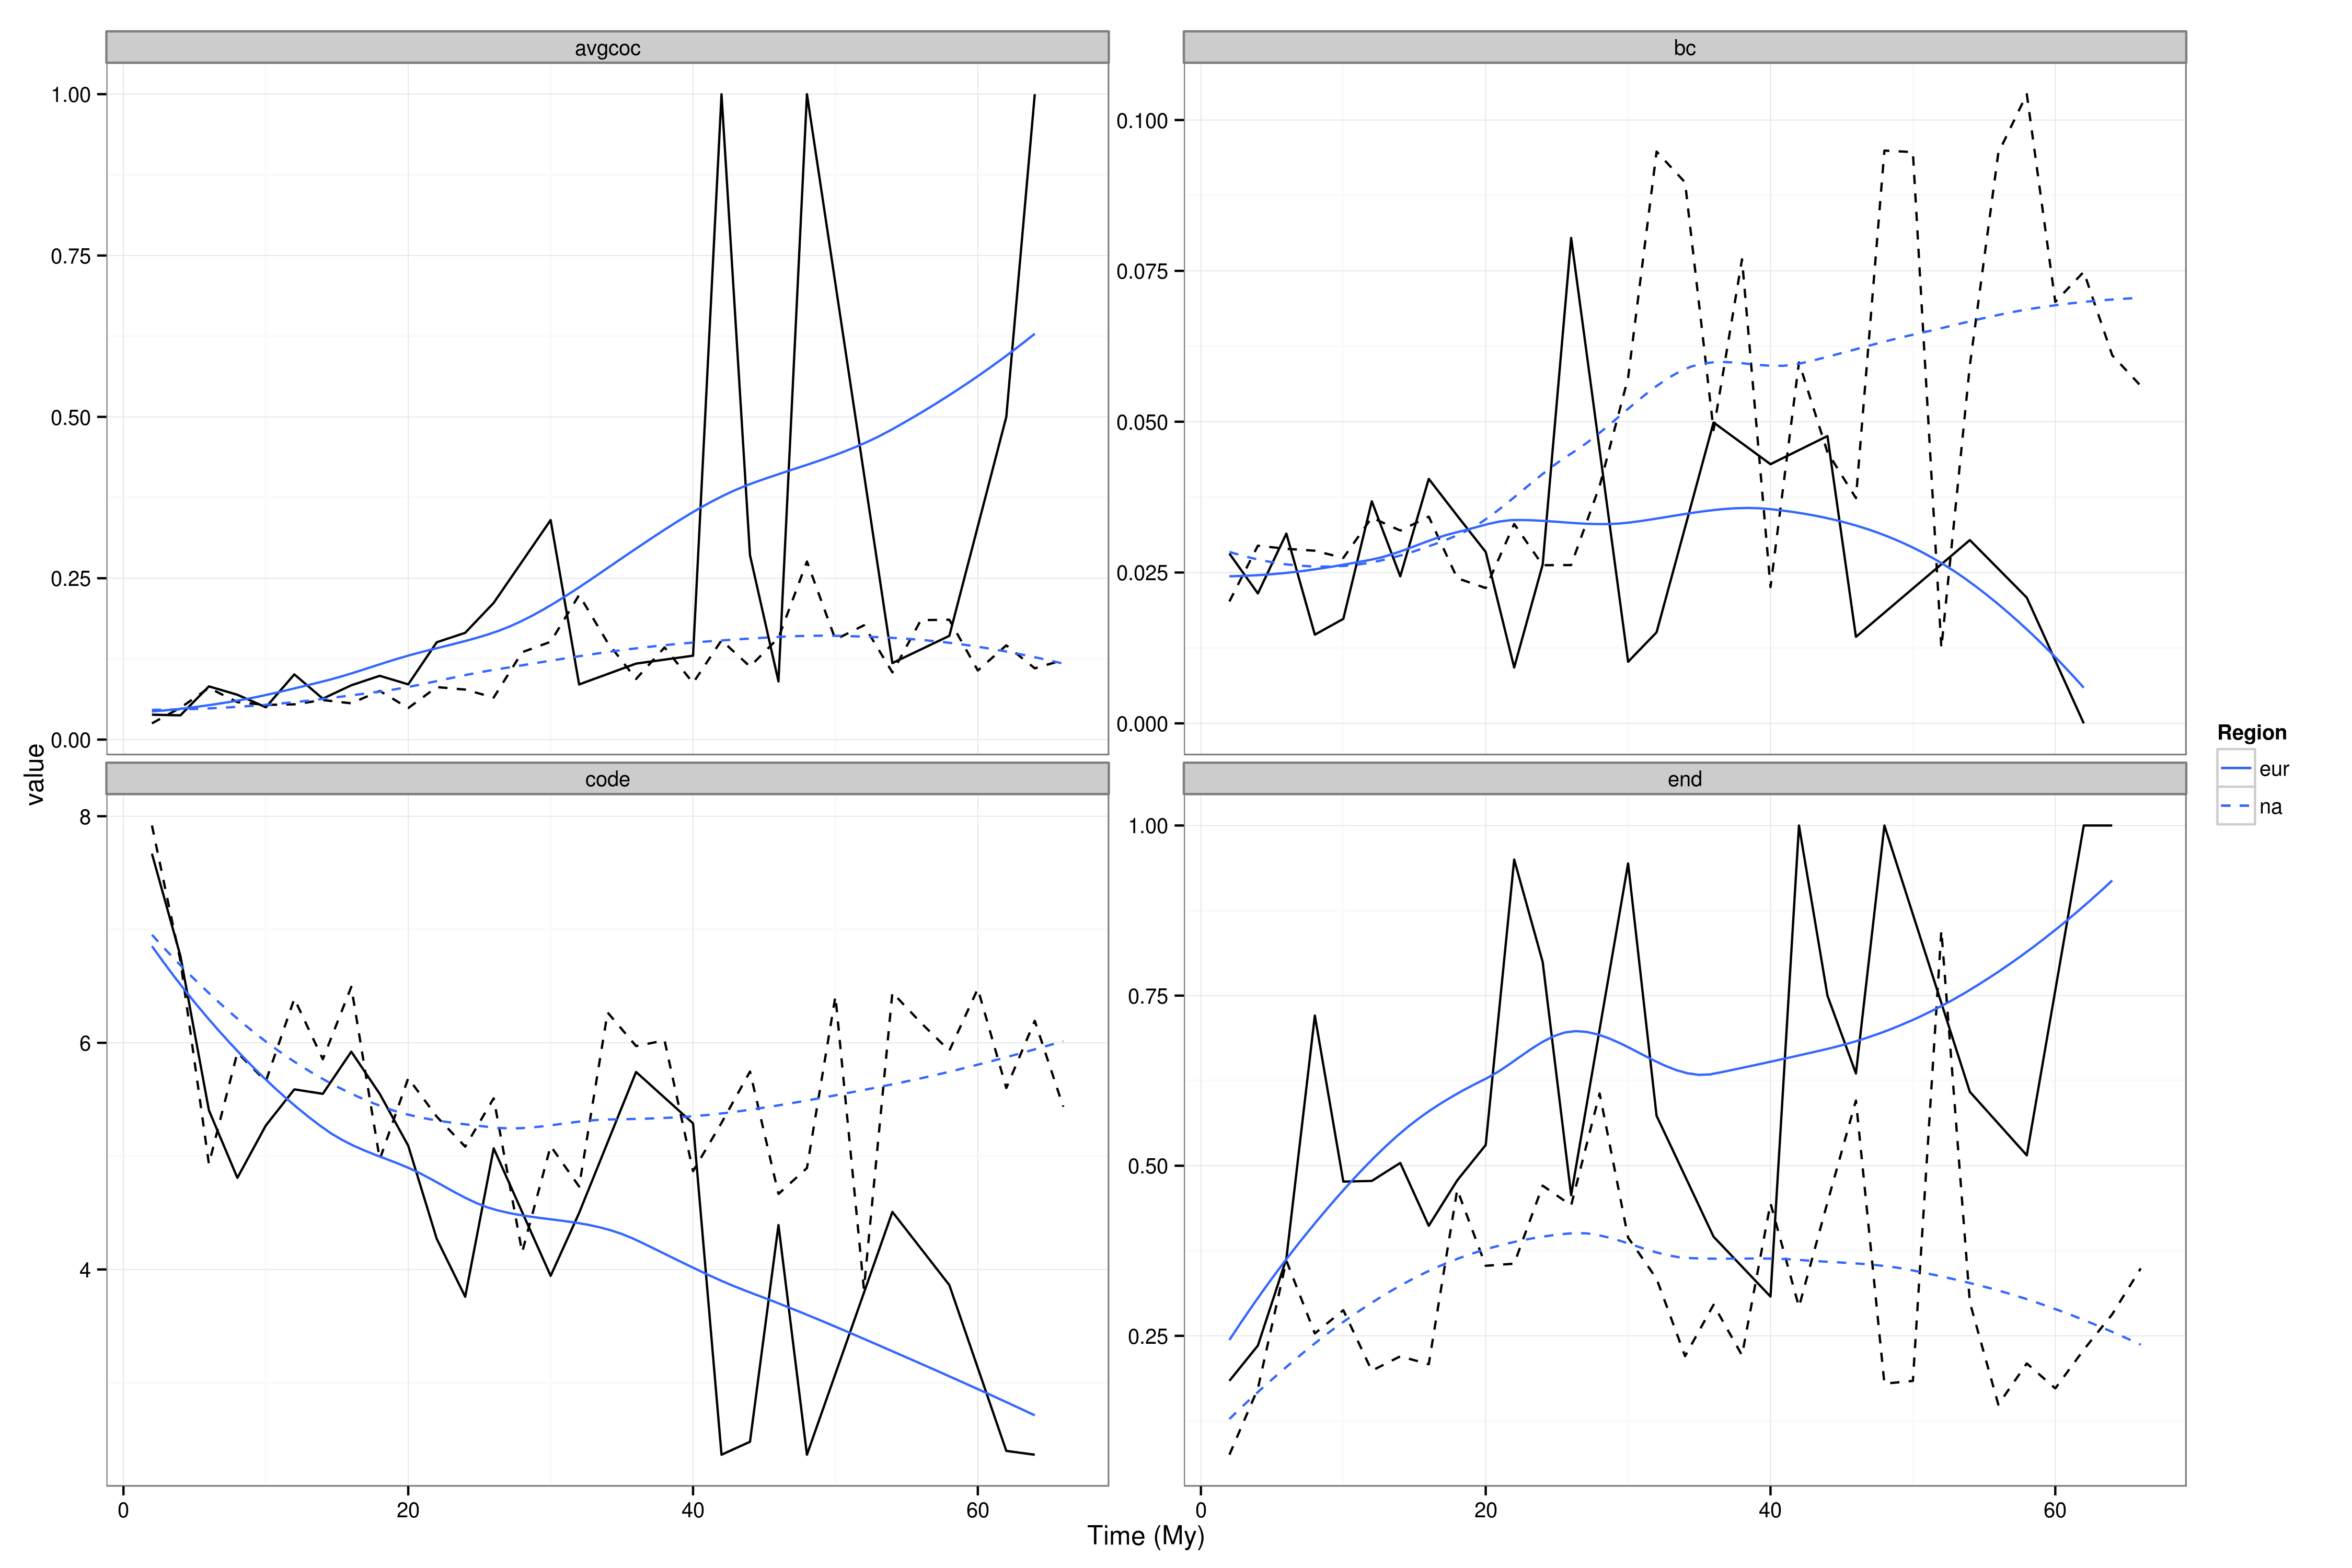
\includegraphics[height = 0.8\textheight, width = \textwidth, keepaspectratio = true]{figure/gen_bin}
  \end{center}
\end{frame}

\begin{frame}
  \frametitle{Preliminary results: locomotor category NA}

  \begin{center}
    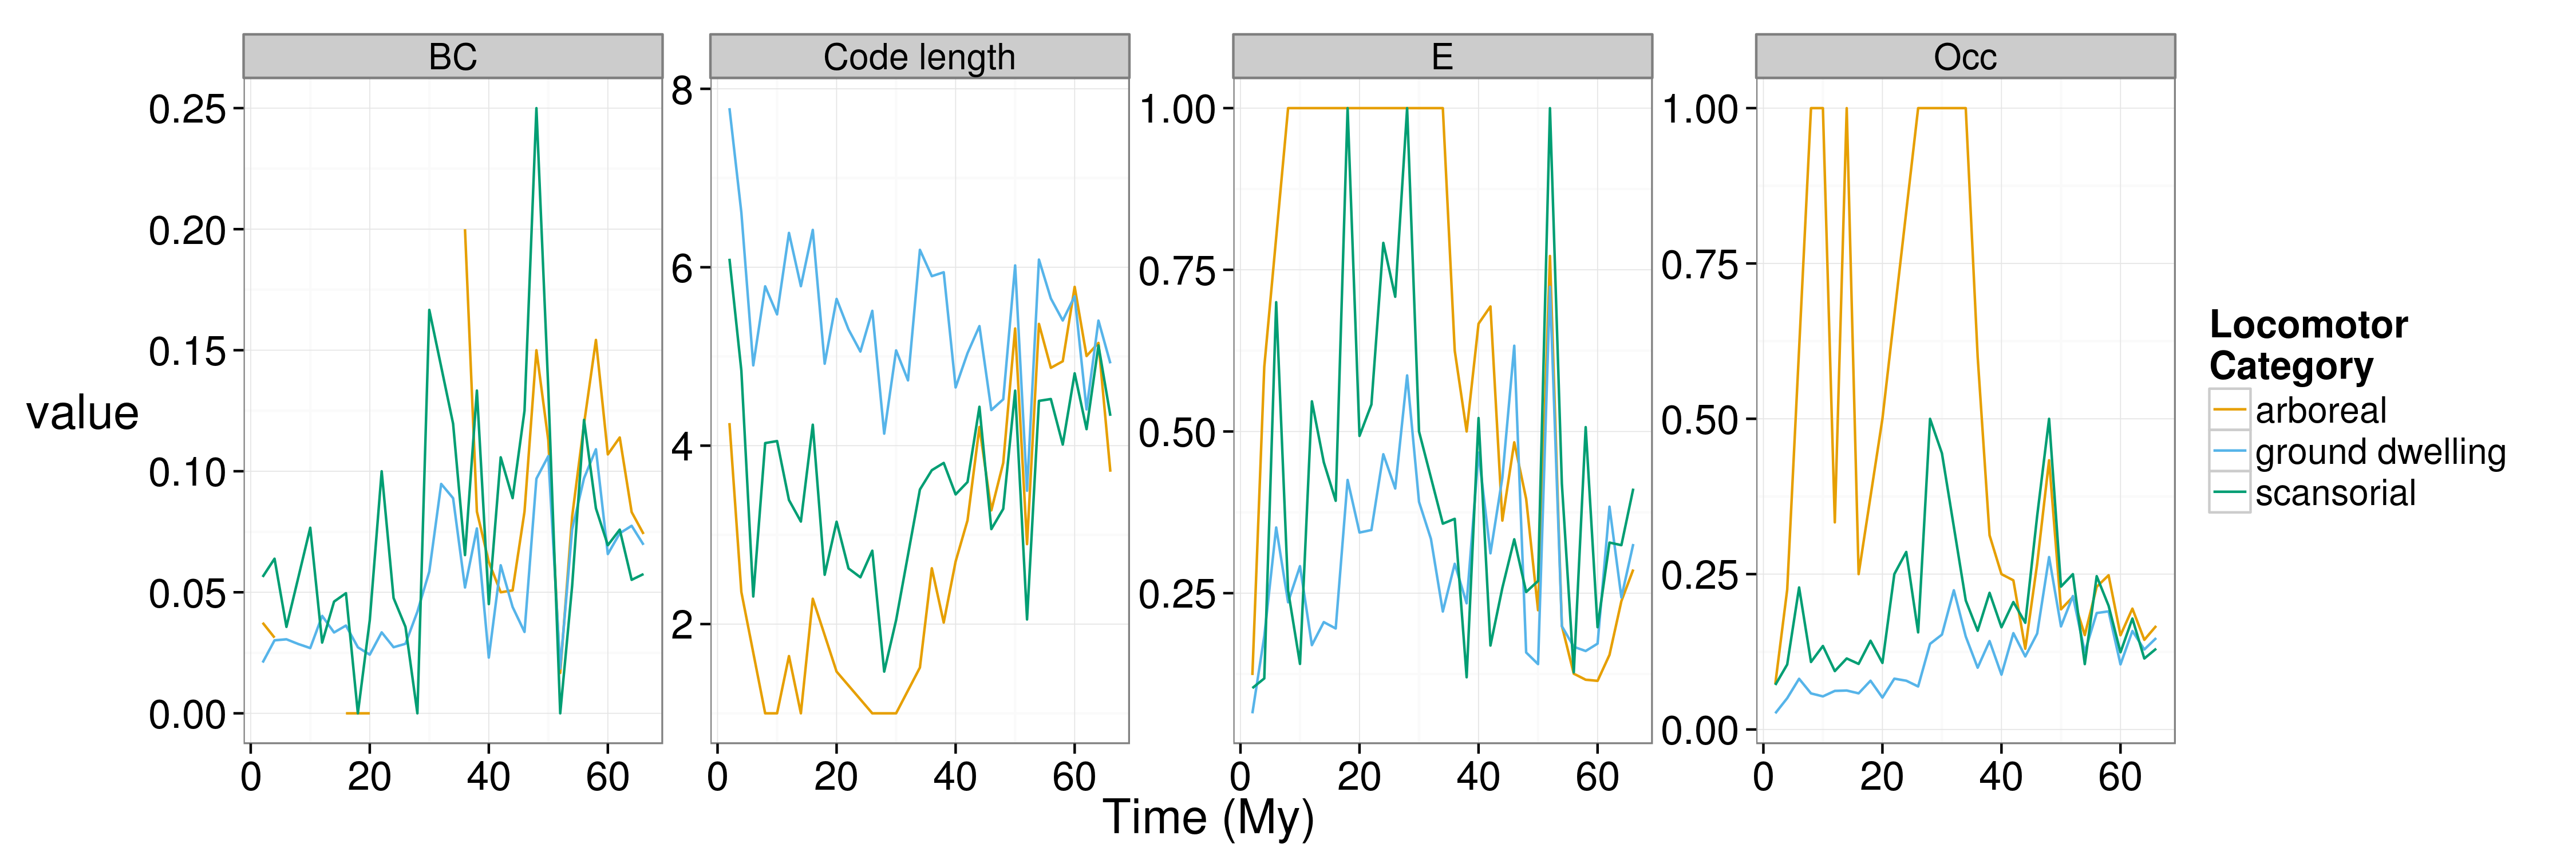
\includegraphics[height = 0.8\textheight, width = \textwidth, keepaspectratio = true]{figure/na_lf}
  \end{center}
\end{frame}

\begin{frame}
  \frametitle{preliminary results: locomotor category Eur}

  \begin{center}
    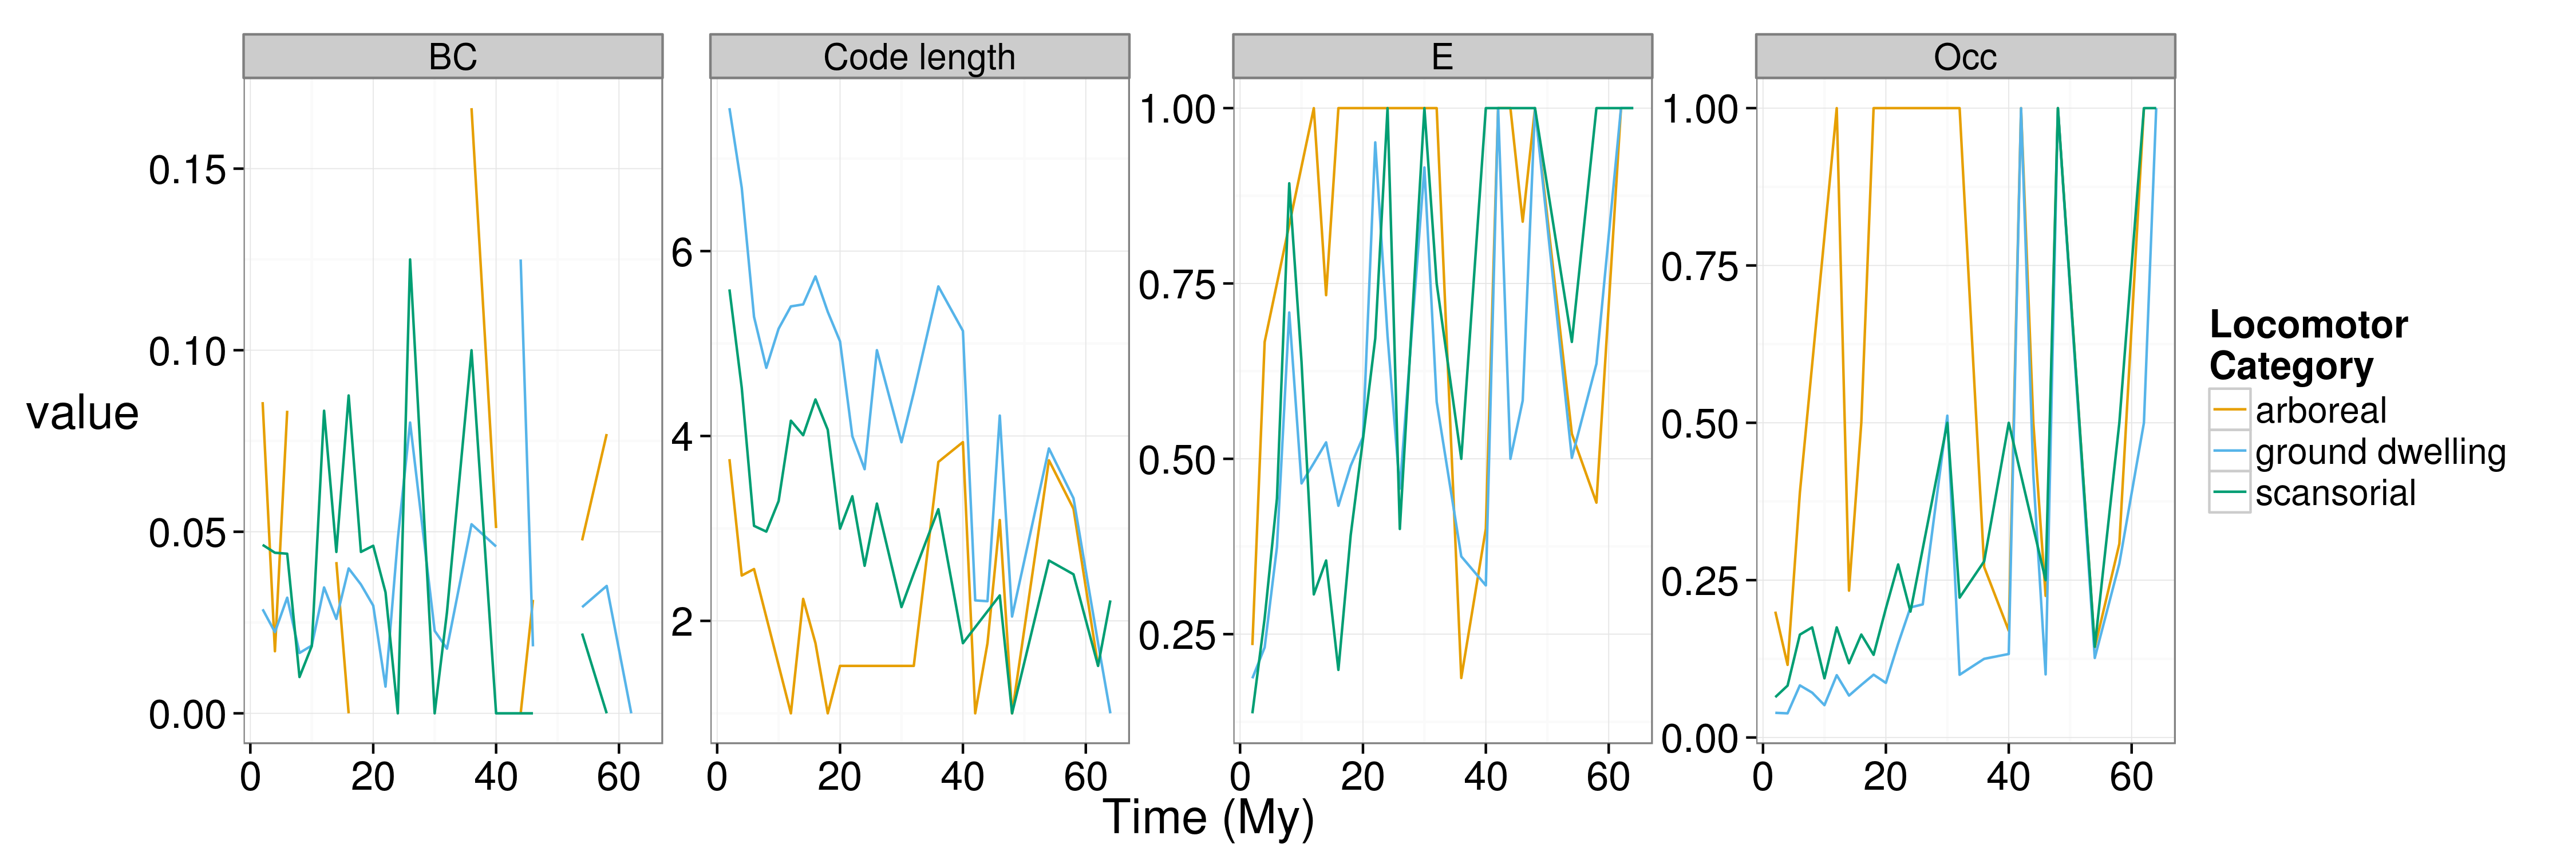
\includegraphics[height = 0.8\textheight, width = \textwidth, keepaspectratio = true]{figure/er_lf}
  \end{center}
\end{frame}

\begin{frame}
  \frametitle{Preliminary results: dietary category NA}

  \begin{center}
    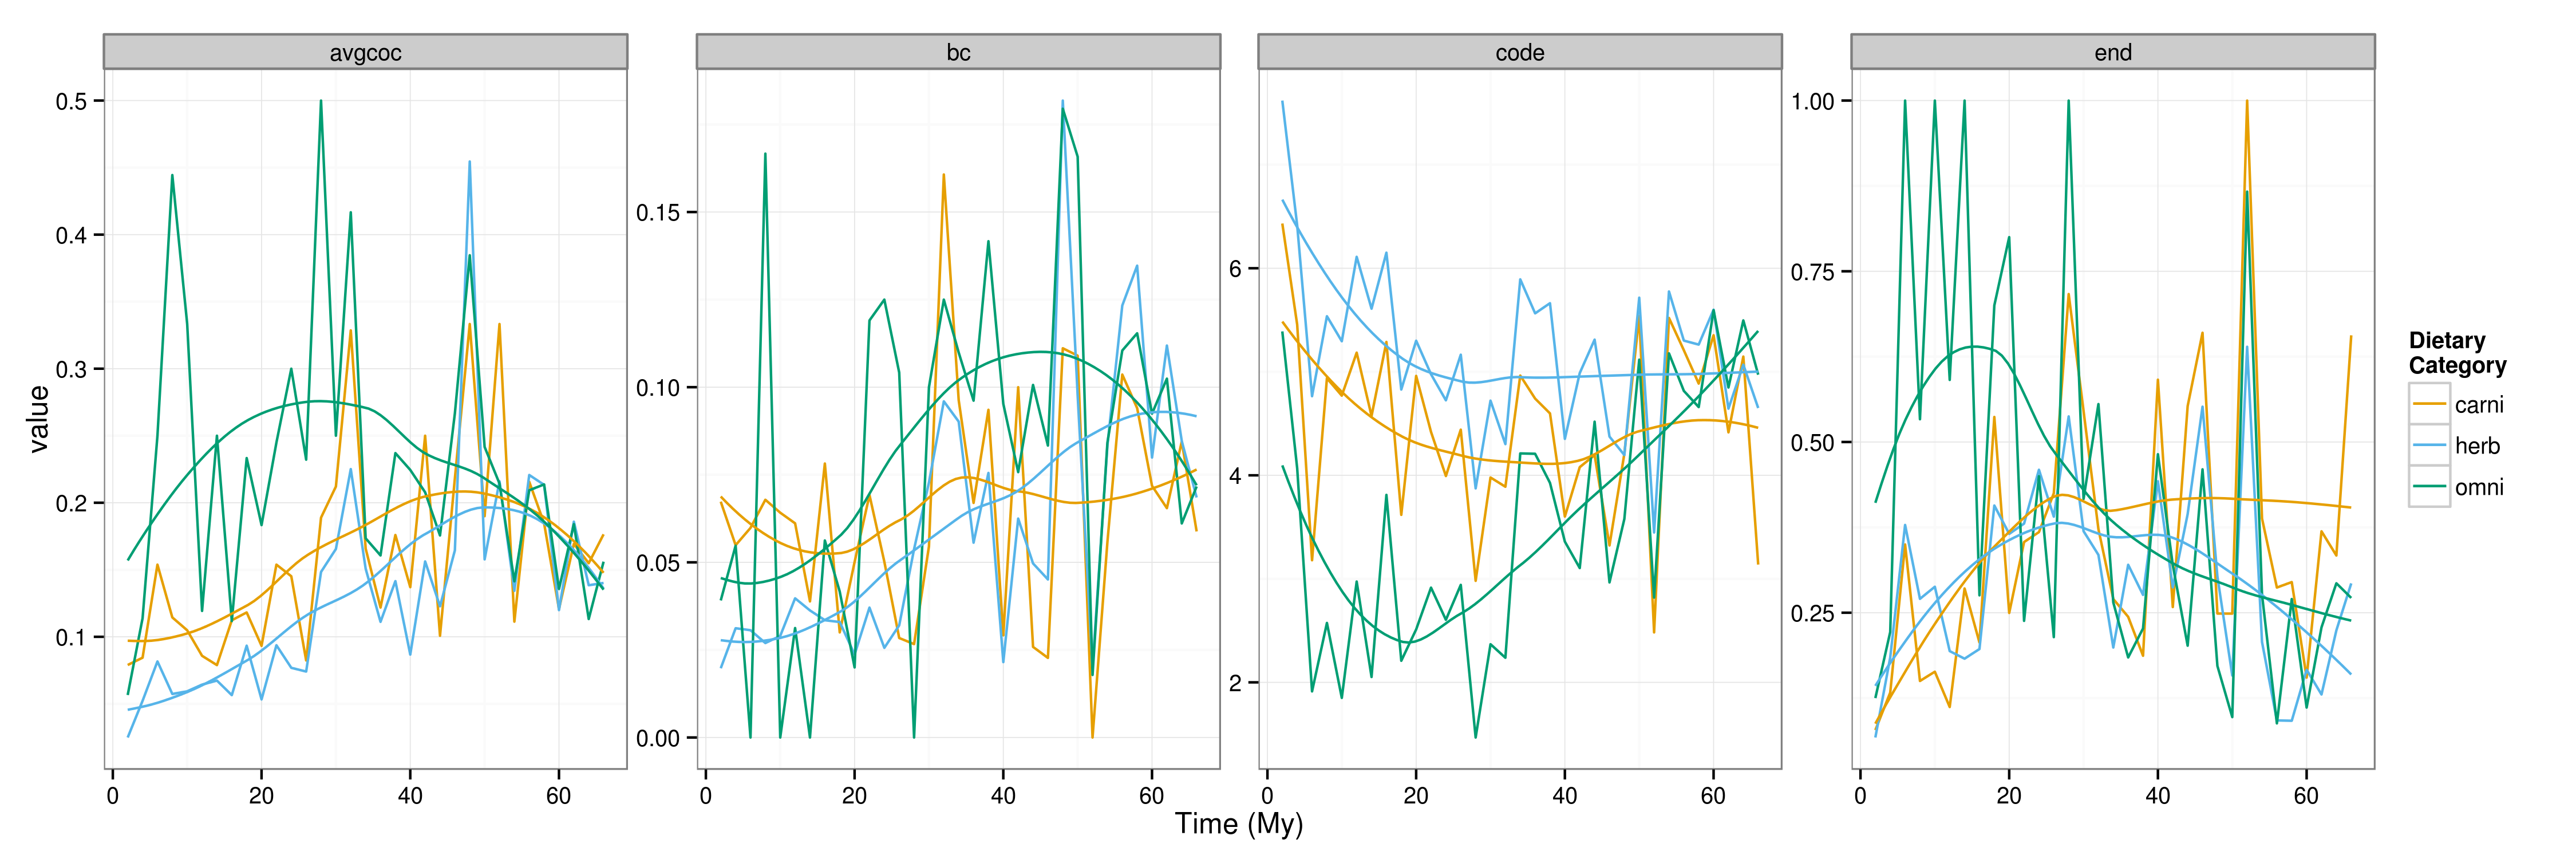
\includegraphics[height = 0.8\textheight, width = \textwidth, keepaspectratio = true]{figure/na_dt}
  \end{center}
\end{frame}

\begin{frame}
  \frametitle{Preliminary results: dietary category Eur}

  \begin{center}
    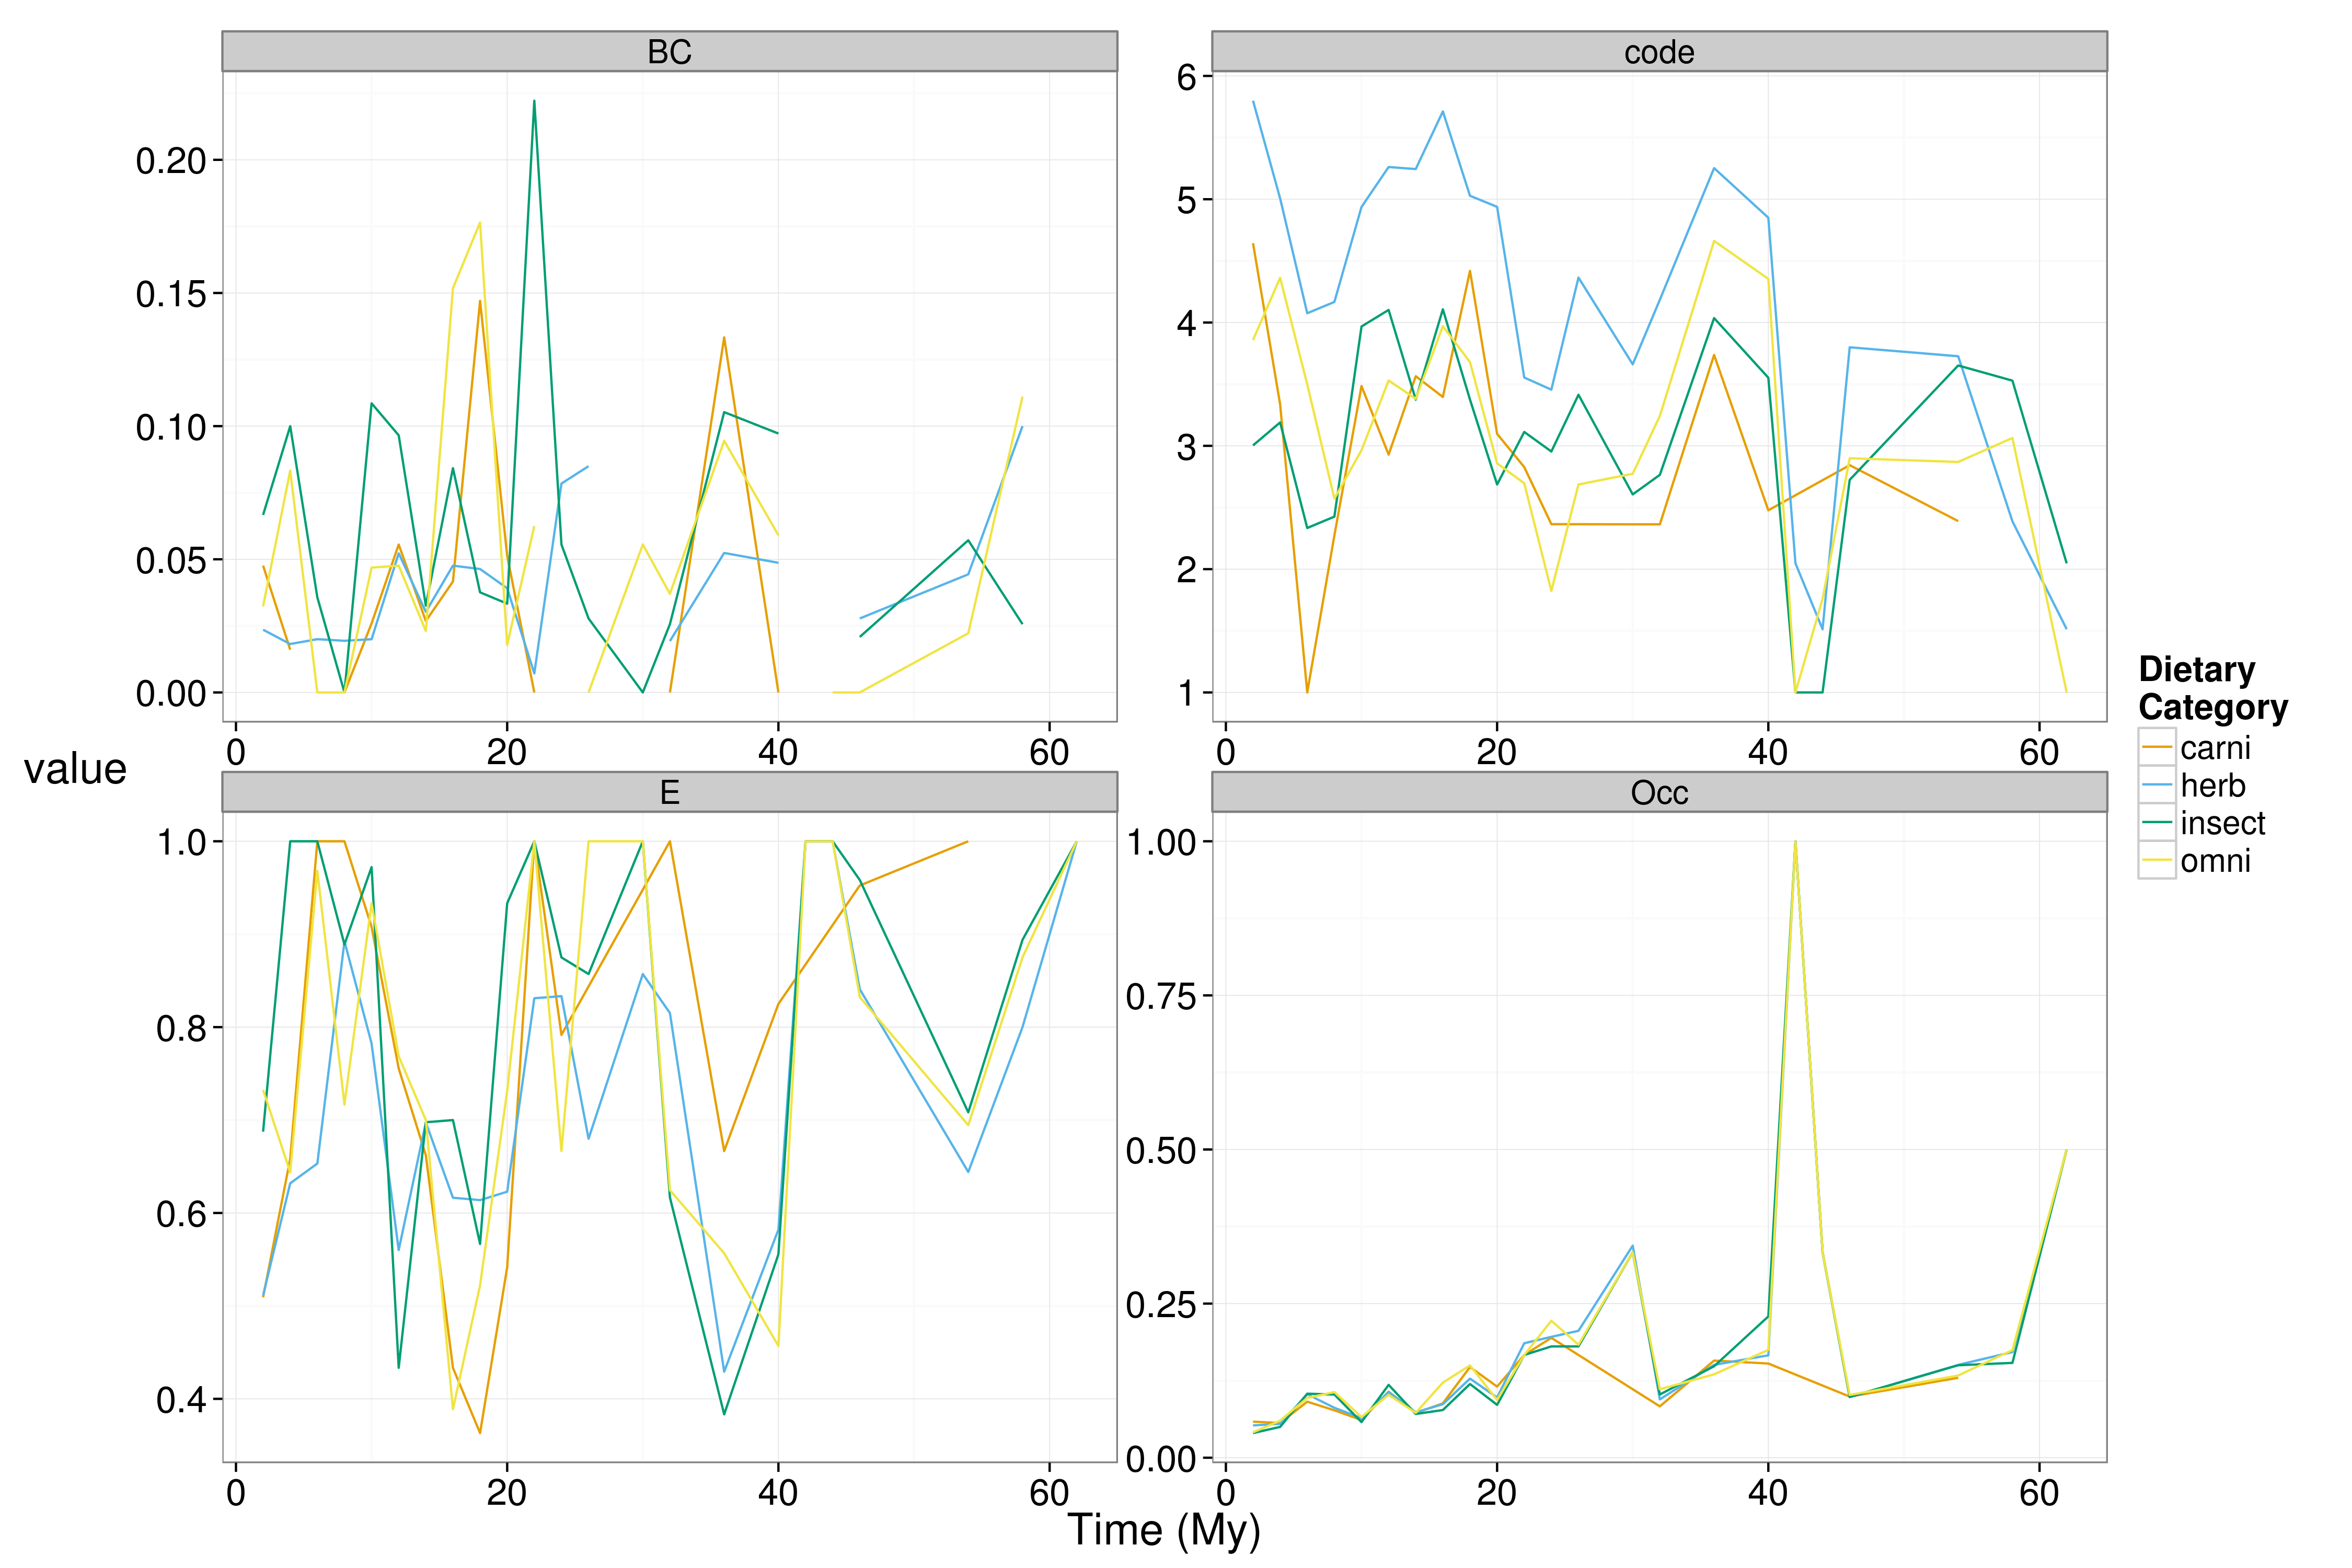
\includegraphics[height = 0.8\textheight, width = \textwidth, keepaspectratio = true]{figure/er_dt}
  \end{center}
\end{frame}


% summary
\begin{frame}
  \frametitle{Questions}

  \begin{alertblock}{Questions}
    \begin{itemize}
      \item Why do certain taxa go extinct while others do not?
      \item How is emergence ``formed?'' When should it be invoked?
      \item Is extinction rate taxon--age independent?
      \item When should we expect global, regional, or local processes to dominate?
    \end{itemize}
  \end{alertblock}
\end{frame}

\begin{frame}
  \frametitle{Summary of proposed research}

  \begin{alertblock}{Studies}
    \begin{itemize}
      \item Permian brachiopod trait based survival %\\(environmental preference)
      \item Cenozoic mammal trait based survival %\\(range size)
      \item Cenozoic mammal community connectedness %\\(global versus regional versus local)
    \end{itemize}
  \end{alertblock}

\end{frame}


\begin{frame}
  \frametitle{Acknowledgements}
  \begin{columns}
    \begin{column}{0.5\textwidth}
      \begin{itemize}
        \item \textbf{Committee}
          \begin{itemize}
            \item Kenneth D. Angielczyk (co-advisor)
            \item Michael J. Foote (co-advisor)
            \item P. David Polly
            \item Richard H. Ree
          \end{itemize}
        \item Discussion
          \begin{itemize}
            \item David Bapst, Megan Boatright, Ben Frable, Colin Kyle, Darcy Ross, Liz Sander
            \item John Alroy, Graeme Lloyd, Carl Simpson, Graham Slater
          \end{itemize}
      \end{itemize}
    \end{column}
    \begin{column}{0.5\textwidth}
      
\includegraphics[height = 0.3\textheight, keepaspectratio = true]{figure/chicago} \\
      
\includegraphics[height = 0.3\textheight, width = 0.5\textwidth, keepaspectratio = true]{figure/field} \\
    \end{column}
  \end{columns}
\end{frame}



\appendix
\section{Further concerns}

\begin{frame}
  \frametitle{Theseus' ship: biases to analyzing survival}

  \begin{columns}
    \begin{column}{0.5\textwidth}
      \begin{center}
        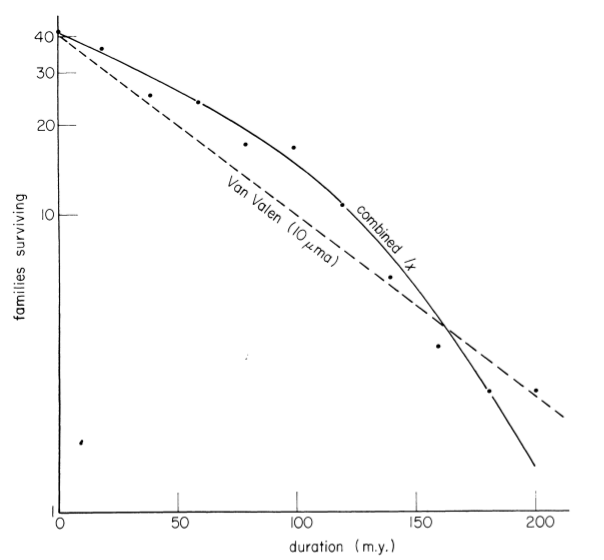
\includegraphics[height = 0.4\textheight, width = \textwidth, keepaspectratio = true]{figure/raup}
          
        \tiny{\attrib{Raup 1975 \textit{Paleobio.}}}

        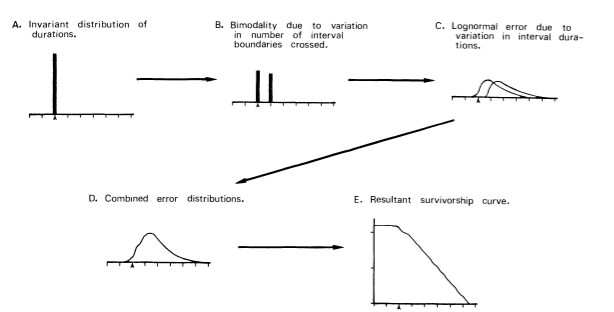
\includegraphics[height = 0.4\textheight, width = \textwidth, keepaspectratio = true]{figure/sepkoski}
          
        \tiny{\attrib{Sepkoski 1975 \textit{Paleobio.}}}
      \end{center}
    \end{column}
    \begin{column}{0.5\textwidth}
      \begin{itemize}
        \item bias away from \(h(t) = \lambda\)?
          \begin{itemize}
            \item censoring
            \item sampling/stratigraphy
            \item species vs genus
            \item anagenesis/cryptic speciation
          \end{itemize}
        \item use time-homogeneous birth-death model
          \begin{itemize}
            \item constant \(p\), \(b\)
            \item expected \(S(t) = \exp^{-\lambda t}\)
            \item vary anagenesis/sampling
          \end{itemize}
      \end{itemize}
    \end{column}
  \end{columns}
\end{frame}

\begin{frame}
  \frametitle{Phylogeneic similarity of communities}

  \begin{columns}
    \begin{column}{0.5\textwidth}
      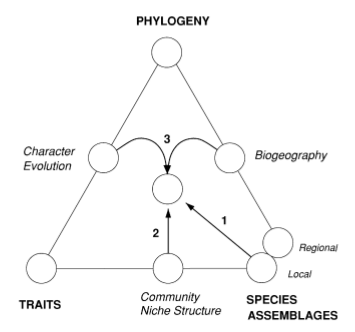
\includegraphics[height = 0.8\textheight, width = \textwidth,  keepaspectratio = true]{figure/webb}

      \tiny{\attrib{Webb \textit{et al.} 2002 \textit{Ann. Rev. Ecol. Syst.}}}
    \end{column}
    \begin{column}{0.5\textwidth}
      \begin{itemize}
        \item informal phylogeny \\(taxonomy tree)
          \begin{itemize}
            \item PBDB, EoL, etc.
            \item unit branch length
          \end{itemize}
        \item measures
          \begin{itemize}
            \item mean pairwise--locality patristic distance
            \item mean locality phylogenetic species variability (Helmus \textit{et al.} 2007 \textit{Am. Nat})
          \end{itemize}
      \end{itemize}
    \end{column}
  \end{columns}
\end{frame}


\end{document}
